\documentclass[11pt]{article}

\usepackage{comment} % enables the use of multi-line comments (\ifx \fi) 
\usepackage[a4paper,margin=1cm]{geometry}
\usepackage[utf8]{inputenc}
\usepackage[ngerman]{isodate}
\usepackage{gensymb}
\usepackage{graphicx}
\usepackage{booktabs}% http://ctan.org/pkg/booktabs
\usepackage{tabularx}
\usepackage{ltablex} % Longtables with tabularx
\usepackage[x11names]{xcolor}
\usepackage{amsmath}
\usepackage{amssymb}
\usepackage{amsthm}
\usepackage{array}
\usepackage{wrapfig}
\usepackage{subcaption}
\usepackage{csquotes}
\usepackage{lscape}
\usepackage{geometry}
\usepackage{multicol}
\usepackage{bm}
\usepackage{enumitem}
\usepackage{hyperref}
\usepackage{mdframed}
\usepackage{scalerel}
\usepackage{stackengine}
\usepackage{mathtools}
\usepackage{pdfpages}

% Code highlighting
\usepackage{minted}
\surroundwithmdframed{minted}

% Be able to caption equations and float them in place
\usepackage{float}

\newmdtheoremenv{theorem}{Theorem}

\theoremstyle{definition}
\newmdtheoremenv{definition}{Definition}[section]

\geometry{a4paper, margin=2.4cm}

\newcommand\equalhat{\mathrel{\stackon[1.5pt]{=}{\stretchto{\scalerel*[\widthof{=}]{\wedge}{\rule{1ex}{3ex}}}{0.5ex}}}}
\newcommand\defeq{\mathrel{\overset{\makebox[0pt]{\mbox{\normalfont\tiny def}}}{=}}}
\newcolumntype{C}{>{\centering\arraybackslash}X}

\DeclarePairedDelimiter\abs{\lvert}{\rvert}
\DeclarePairedDelimiter\norm{\lVert}{\rVert}

\setcounter{tocdepth}{3}
\setcounter{secnumdepth}{3}

\graphicspath{{./img/}}

\begin{document}
	
\title{Private Law FS20}
\author{Pascal Baumann\\pascal.baumann@stud.hslu.ch}
\maketitle



For errors or improvement raise an issue or make a pull request on the \href{https://github.com/KilnOfTheSecondFlame/mse_summaries}{github repository}.

\tableofcontents
\newpage



\section{Introduction}
The goal of the module is to foster an understanding on the different dimensions of privacy and a thinking in the corresponding contexts. Transferring privacy aspects to
and within the private and work environment and reflecting upon these, establishing links with learning content in the MRU and the technical modules. Acquiring an appreciation of the legal aspects confronting an engineer in demanding professional situations. Gaining awareness in order to avoid damages due to infringements of rights or legal uncertainty. Acquisition of speaking and listening
skills in order to conduct the corresponding specialist discussions with experts.

Law is a social framework, that saves energy by providing an orientation how to manage conflicts and preserve the values of the culture the law was created in. The law legitimises public authorities and courts, and aims to control the power inherent in any system so that no imbalance is present. 

\subsection{Importance of Law in a Technical or Information Technology World}

The law provides a guideline of the allowed/maximum or obligatory requirement/minimum a system has to satisfy. It clarifies obligations, responsibilities and liability. Industry standards apply the law to a specific field, although they do not clear all legal questions most of the time.

In risk management not only technical or organisational risks have to be considered, but also legal measures to mitigate risks. It is prudent to consult legal as soon as possible in a project, otherwise it may be stopped at the last minute and be very costly. By law, management is responsible that an organisation complies to the legal framework.

\subsection{Importance of Privacy and Personal Data Protection}
Personal data in the wrong hands may harm the person in question in various forms. Privacy and the \emph{right to forget} is essential in personal development. An owner with a big collection of such personal data gets a lot of power with little oversight or control. One of the main tasks of a state is to protect its citizen, this includes protection from attacks on personal data.

\paragraph{One of the Most Vital Legal Questions}
\begin{definition}
	{\scriptsize (1)} \textbf{Who} wants from {\scriptsize (2)} \textbf{whom} {\scriptsize (3)}\textbf{what} based on what {\scriptsize (4)}\textbf{title} or right?
\end{definition}

\begin{figure}[H]
	\centering
	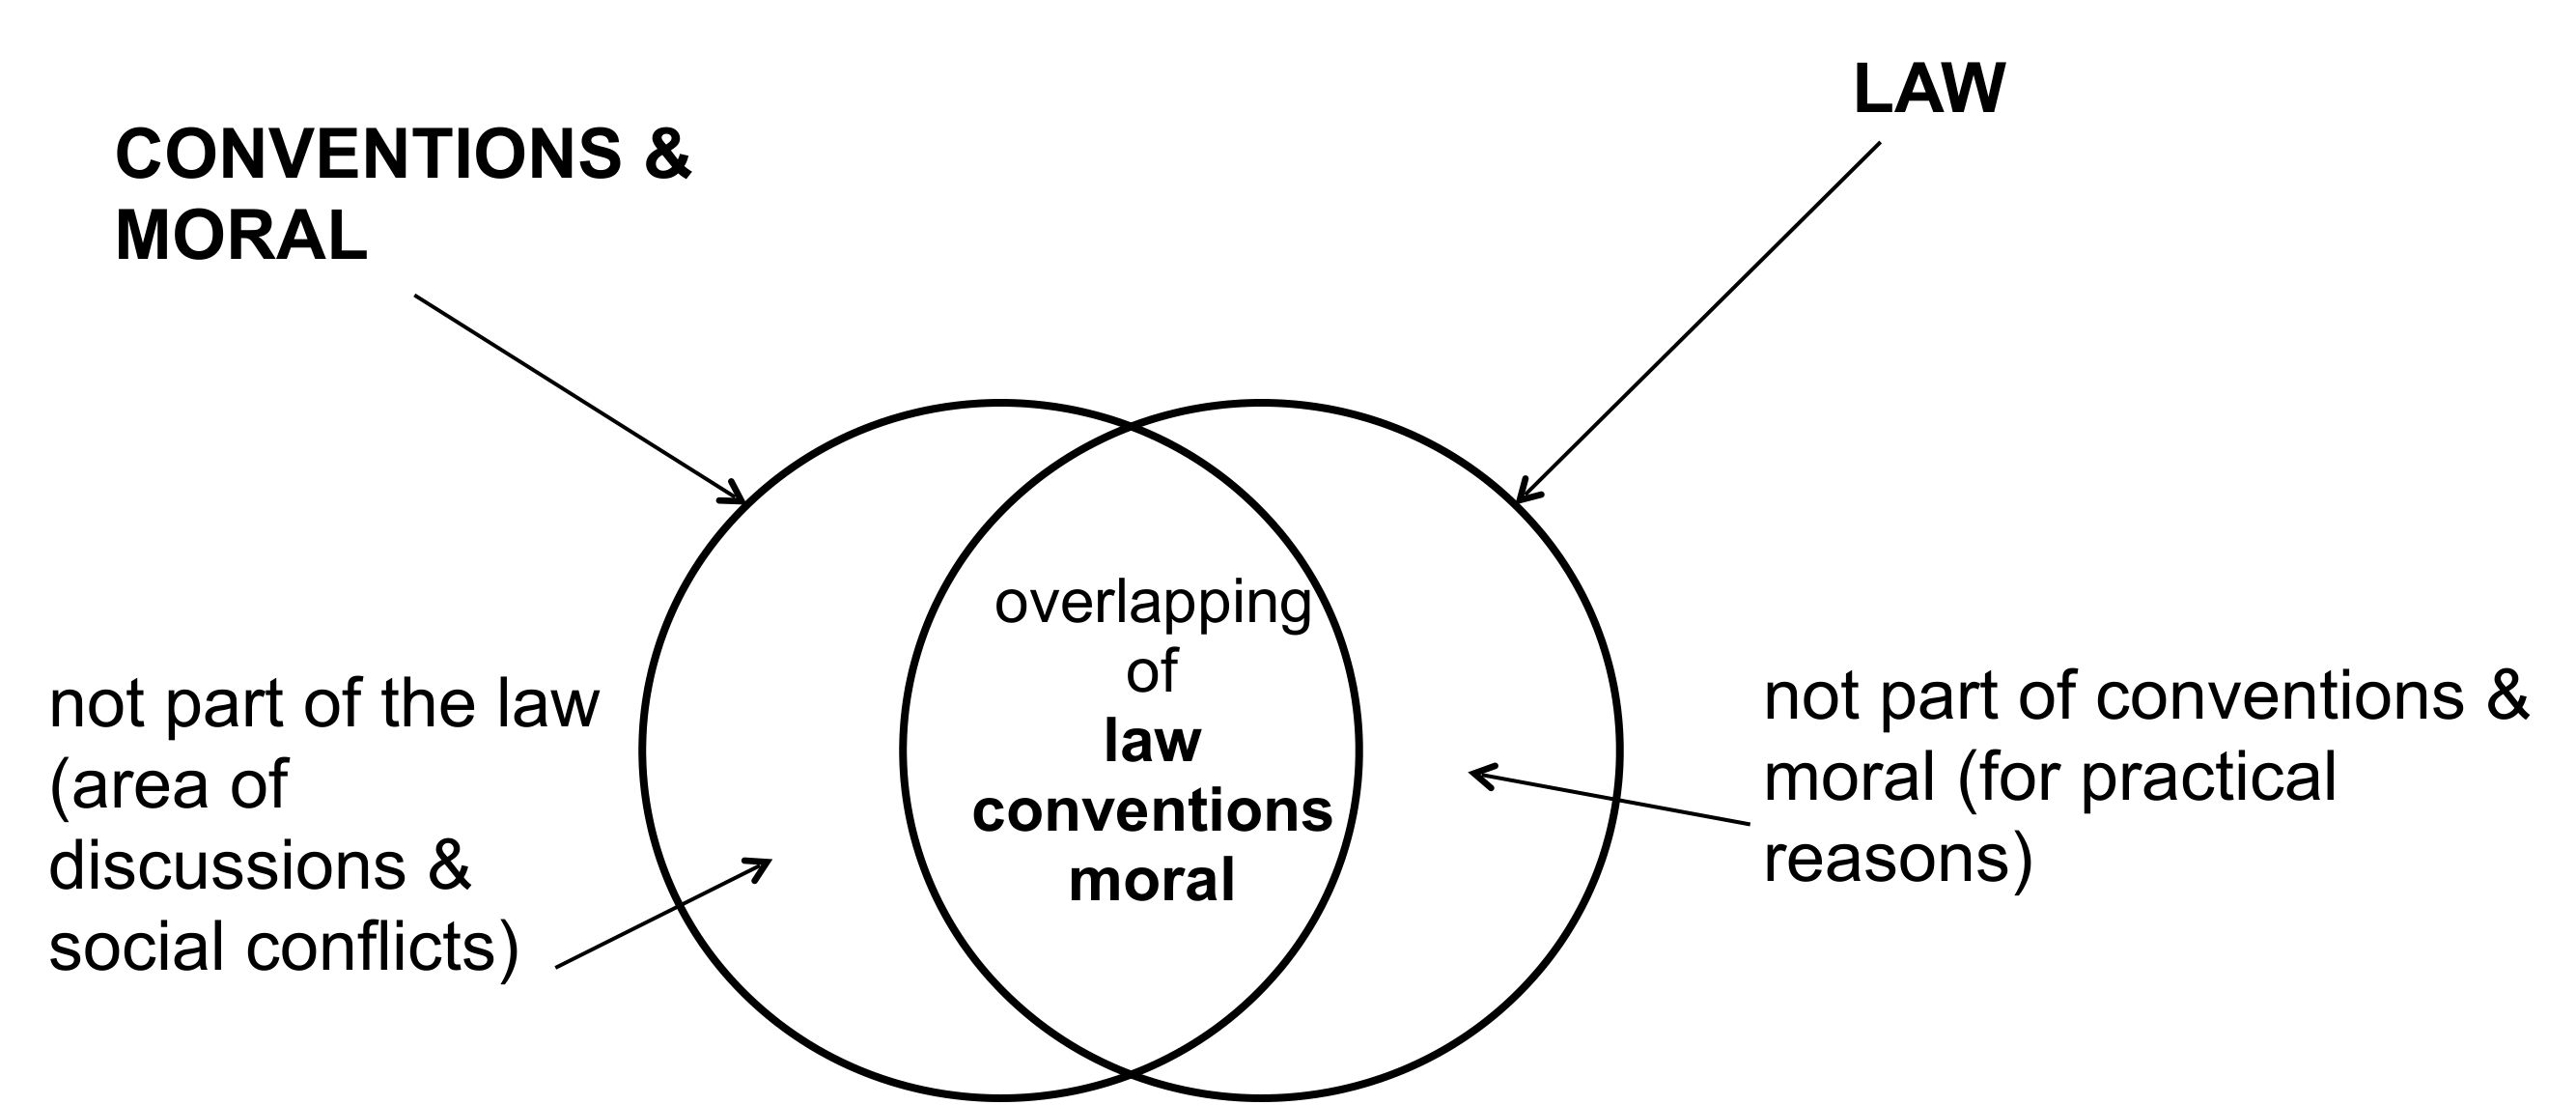
\includegraphics[width=0.8\linewidth]{img/conventions_moral_law}
	\caption{The relationship between conventions, morals and law}
	\label{fig:conventionsmorallaw}
\end{figure}

\subsection{Correct Legal Argumentation}
A statement or claim has to be justified by legal articles or arguments and the necessary evidence. Or is based on legal articles or arguments and with the necessary evidence arrives at a conclusion.

The law get classified by
\begin{itemize}
	\item Status: constitution, act, regulations or by-law
	\item Issuer: Federal, Cantonal and Communal Law
	\item Source of the Law: written law, common law, judicial tradition
	\item Involved Person: Civil Law or Public Law
\end{itemize}

At each of the federal, cantonal and communal level there is a separation of power into the \textbf{legislative}, the \textbf{executive} and the \textbf{Judiciary}, which provides a check and balance on the power of each authority.

\subsection{State, Cantons, Communes}

"Das Schweizervolk und die Kantone [...] bilden die Schweizerische Eidgenossenschaft", (1. Art BV).

"Der Kanton arbeitet mit den Gemeinden, den anderen Kantonen, dem Bund und, in seinem Zuständigkeitsbereich, mit dem Ausland zusammen." Therefore the State is only entitled to legislate and act in a territory or legal field where it has a constitutional legitimacy. The cantons are superior to the state in their power of legislation.

\begin{center}
	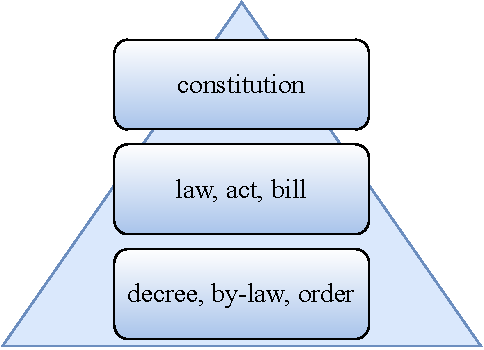
\includegraphics[width=0.4\linewidth,keepaspectratio]{law_hierarchy}
\end{center}

\begin{tabularx}{\linewidth}{X|X}
	\textbf{civil law} & \textbf{public law}\\
	\hline
	OR/ZGB & StGB\\
	GeBüV & FMG\\
	DSG & BÜPF/VÜPF\\
	URG, UWG & EIDI-V\\
	\vdots & \vdots
\end{tabularx}

Civil law is mastered by the \textbf{principle of freedom} of coalition and freedom of contract. Public law is mastered by the \textbf{principle of legality}, the control of power. This results in completely different jurisdictions with different procedures and rights for each.

\subsection{By-Law (Verordnung) $\neq$ Order (Verfügung)}

A By-Law is a \textbf{general, abstract regulation} as part of a law, while an order is an \textbf{individual, concrete application} of a law to a person.

\subsection{Legal Terms}
\begin{itemize}
	\item mandatory rules, stipulated rules and dispositive rules
	\item bona fide or good faith (ZGB 2)
	\item acting in good faith or a fair manner
	\item judicial discretion (ZGB 4)
	\item burden of proof (ZGB 8)
\end{itemize}

\subsection{International Law Framework}
Switzerland is integrated into the European legal framework by long-time traditions, unilateral and bilateral conventions. The IPRG ("Gesetz über das internationale Privatrecht") specifies the bridge between Swiss and foreign law. It rules which law is applicable and which court is competent. Parties can decide in most cases, under which jurisdiction they want to handle their disputes and which court will be competent.

There are generally three different instances in these jurisdictions:
\begin{itemize}
	\item Bezirksgericht
	\item Kantonsgericht
	\item Bundesgericht
\end{itemize}

\section{Copyright}
Through applying creative intellect a work is created. This work enjoys copyright, which means the creator may decide how this work is distributed. Copyright law guarantees them financial remuneration for the utilisation of their works. Moreover, the copyright law protects artists’ intellectual property in that they are able to defend themselves against
misappropriation of their work. Creative endeavour is a public good. Intellectual creations are the driving force of our economy.

\subsection{Prerequisites for Legal Protection of a Work}
A work must be an \textbf{intellectual creation} and have \textbf{Statistical Uniqueness}:
\begin{itemize}
	\item Individual character, characteristic features
	\item Sufficiently creative step, work is special and unique
\end{itemize}

There must be a perceptibility or expression of an idea. And ultimately a work must be created by humans.

With the new law all photographs and reproductions produced by similar methods of three-dimensional objects (film stills) will be subject to copyright protection.

\paragraph{Art 3 Swiss Copyright Act - Derivative Works}
\begin{enumerate}[label=\arabic* ]
	\item Derivative works are intellectual creations with an individual character that are \textbf{based upon pre-existing works, whereby the individual character of the latter remains identifiable.}
	\item Such works include, in particular, \textbf{translations} as well as audio-visual and other \textbf{adaptations}.
	\item Derivative works are protected as \textbf{works in their own right}.
	\item The protection of the works used in the derivative work remains reserved.
\end{enumerate}

To create a derivative work you require the consent of the copyright owner of the original work.

\subsection{Non-derivative Works}
\begin{enumerate}[label=\arabic* ]
	\item \textbf{rework}
	\begin{itemize}
		\item use of pre-existing works
		\item mere rework of an original work, no individual character
	\end{itemize}
	\item \textbf{new creation}
	\begin{itemize}
		\item original work is merely an inspiration and cannot be recognised or identified in the new creation
		\item the newly created work is protected individually in its own right
	\end{itemize}
\end{enumerate}

\subsection{Meaning of Copyright}
The \textbf{author of a copyrighted work} is always the natural person who created the work, which is known as \textbf{creator principle}.	Copyright law is an \textbf{absolute right} and thus excludes every other person. Copyrights can be transferred from the \textbf{original author} to another person or legal entity who then becomes the \textbf{right holder}.

\paragraph{Art 9 Swiss Copyright Act}
\begin{enumerate}[label=\arabic*]
	\item The author has the exclusive right to his own work and the right to recognition of his authorship.
	\item The author has the exclusive right to decide whether, when, how and under what author's designation his own work is published for the first time.
	\item A work is considered to be published when it has been made available for the first time by the author, or with his consent, to a large number of persons not constituting a private circle.
\end{enumerate}

\paragraph{Art 10 Swiss Copyright Act}
\begin{enumerate}[label=\arabic*]
	\item \textbf{The author has the exclusive right to decide whether, when and how his work is used.}
	\item The author has the right, in particular:
	\begin{enumerate}[label=\alph*.]
		\item to produce \textbf{copies} of the work, such as printed matter, phonograms, audio-visual fixations or data carriers;
		\item to offer, transfer or otherwise \textbf{distribute} copies of the work;
		\item to recite, \textbf{perform} or present a work, or make it \textbf{perceptible} somewhere else or \textbf{make it available} directly or through any kind of medium in such a way that persons may access it from a place and at a time individually chosen by them;
		\item to \textbf{broadcast} the work by radio, television or similar means, including by wire;
		\item to \textbf{retransmit} works by means of technical equipment, the provider of which is not the original broadcasting organisation, in particular including by wire;
		\item to make works made available, broadcast and retransmitted \textbf{perceptible}.
	\end{enumerate}
	\item The author of a computer program also has the exclusive rental right.
\end{enumerate}

\paragraph{Art 11 Swiss Copyright Act}
\begin{enumerate}[label=\arabic*]
	\item The author has the exclusive right to decide:
	\begin{enumerate}[label=\alph*.]
		\item whether, when and how the work may be \textbf{altered};
		\item whether, when and how the work may be used to create a \textbf{derivative work} or may be \textbf{included in a collected work}.
	\end{enumerate}
	\item Even where a third party is authorised by contract or law to alter the work or to use it to create a derivative work, the author may \textbf{oppose any distortion} of the work that is a violation of his personal rights.
	\item It is permissible to use existing works for the creation of parodies or other comparable variations on the work.
\end{enumerate}

\paragraph{Art 15 Swiss Copyright Act}
\begin{enumerate}[label=\arabic*]
	\item Where the owner of an original work of which no further copies exist has reason to assume that the author of the work has a legitimate interest in its preservation, he may not destroy the work without first offering to return it to the author. The owner may not request more than the material value of the work.
\end{enumerate}

\subsection{Transfer of Copyright}
Moral rights vest in the author and cannot be transferred or licensed, but they may be waived or transferred to heirs upon death.

\textbf{Economic rights may be transferred to third parties and transferred to heirs upon death, use rights may be licensed.}

The transfer of a work or copy of the work does not transfer the rights in the work, even if the original work is transferred.

\subsection{Joint Authorship}
This happen when multiple people \textbf{work together} pursuant to a \textbf{common concept} to create a work together. They can decide jointly on what happens with the work and must all agree to that.

\subsection{Duration of Copyright}
In Switzerland there is an \textbf{automatic protection with no formalities required}. A work is protected under copyright as soon as it is \textbf{created}.

Copyright protection starts as soon as a work is created and the prerequisites
for protection are met. In Switzerland copyright protection expires \textbf{70 years after the death of the author}. The protection for \textbf{computer programs} ends \textbf{50 years after the death of the author}. The protection of \textbf{pictures which do not possess an individual character} ends \textbf{50 years after their creation}.

\subsection{Limitations of Copyright}
\begin{center}
	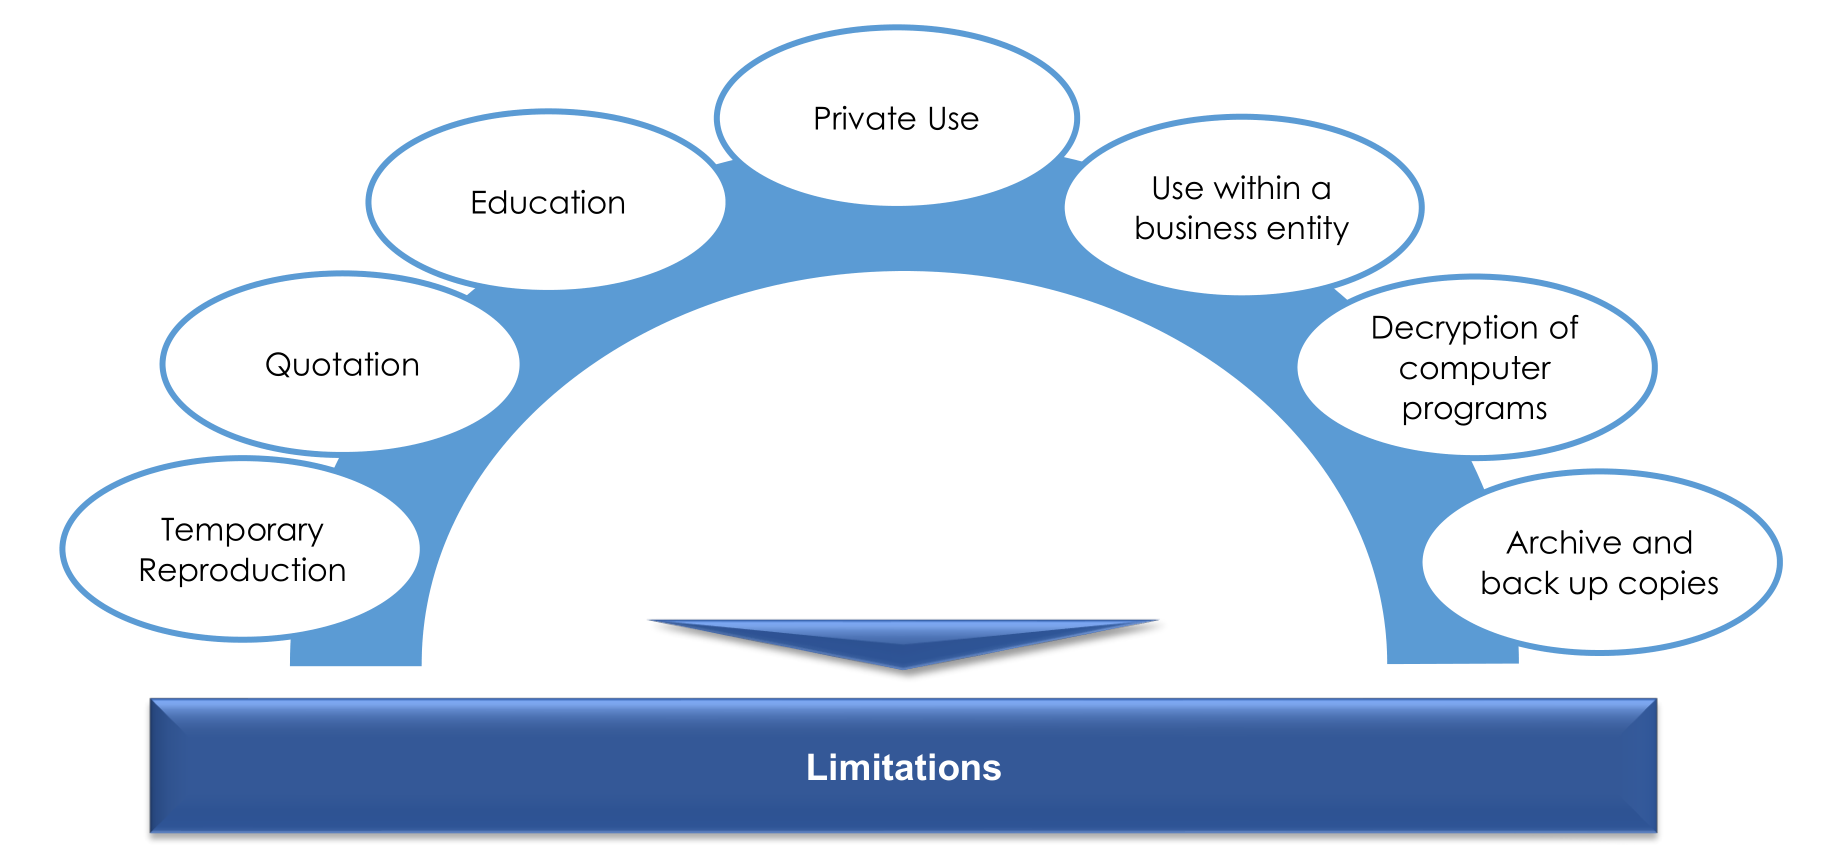
\includegraphics[width=0.8\linewidth]{img/limitations_of_copyright}
\end{center}
Private use includes only the \textbf{use in a private setting for private purposes},
sharing with family and close friends (private circle). \textbf{Private use is not subject to a license fee}. The download of copyrighted works is considered private use. 

\subsection{Related Rights}
The Copyright Act also regulates related rights also referred to as neighbouring rights.
\begin{itemize}[label=-]
	\item rights of \textbf{performing artists} to their performances
	\item rights of \textbf{producers of phonograms and videograms} to their products
	\item rights of \textbf{broadcasters} to their radio and television broadcasts
\end{itemize}

Related rights protection expires \textbf{50 years after the performance}, the publication of the phonogram or videogram or the production of it, in the case that it is not published or the emission of the broadcast.

\subsection{Civil Proceedings}
A copyright claim between private persons or private legal entities are discussed in civil proceedings in a civil court. The \textbf{right holder can request from the civil court}:
\begin{itemize}
	\item a declaratory judgement, that is have a right established
	\item have an infringement banned or remedied
	\item have property confiscated
	\item have an order published
	\item claim damages
\end{itemize}

\subsection{Criminal Proceedings}

Criminal procedures may be initiated by the author / right holder within \textbf{three months} after becoming aware of an infringement or by the authorities, and may result in fines or imprisonment of up to one year (five years if done on a commercial basis).

\begin{itemize}
	\item use of a work within correctly indicating the author
	\item publishing a work
	\item change a work
	\item use for derivative work
	\item copies of works
	\item distributing or making works available
	\item broadcasting
	\item renting out of computer programs
\end{itemize}

\subsection{Collecting Societies}
The Federal Copyright Act is based on the view that the rights accruing to authors are essentially the \textbf{responsibility of the right holders to assert} for themselves.

The Federal Copyright Act only envisages collective management by collective rights management organisations in circumstances where \textbf{mass utilisation makes direct management virtually impossible}. To do so, the collecting societies establish tariffs which are negotiated with the primary user associations.

A comprehensive network of \textbf{reciprocity contracts with affiliated foreign societies} results in an \textbf{exchange} of rights and remunerations. The Swiss societies license the entire world repertoire.

\subsection{Copyright and the Internet}
Downloading, copying, scanning are types of use of a copyrighted work. This permission must be given \textbf{expressly} or \textbf{implied}. Links facilitates access to the page and \emph{implies} to the internet user that the linked pages are \textbf{associated}. Therefore, rights may be \textbf{infringed simply through linking}.

\section{Swiss Personal Data Protection}

\subsection{Reason for Data Protection}
\begin{minipage}{0.6\linewidth}
	Data Protection does not mean protecting data, but protecting people. Humans have a social (public) but also an individual nature (privacy). Human learning imply making faults, and an individual should not be reminded for his faults all his life, there needs to be a right to be forgotten.\\
	
	\vspace{1em}
	\noindent
	\textbf{Protection of Integrity / Personality - Art 28 CC (ZGB)} \\
	\noindent
	Any person whose personality rights are unlawfully infringed may petition the court for protecting against all those causing the infringement.
\end{minipage}
\begin{minipage}{0.4\linewidth}
	\begin{center}
		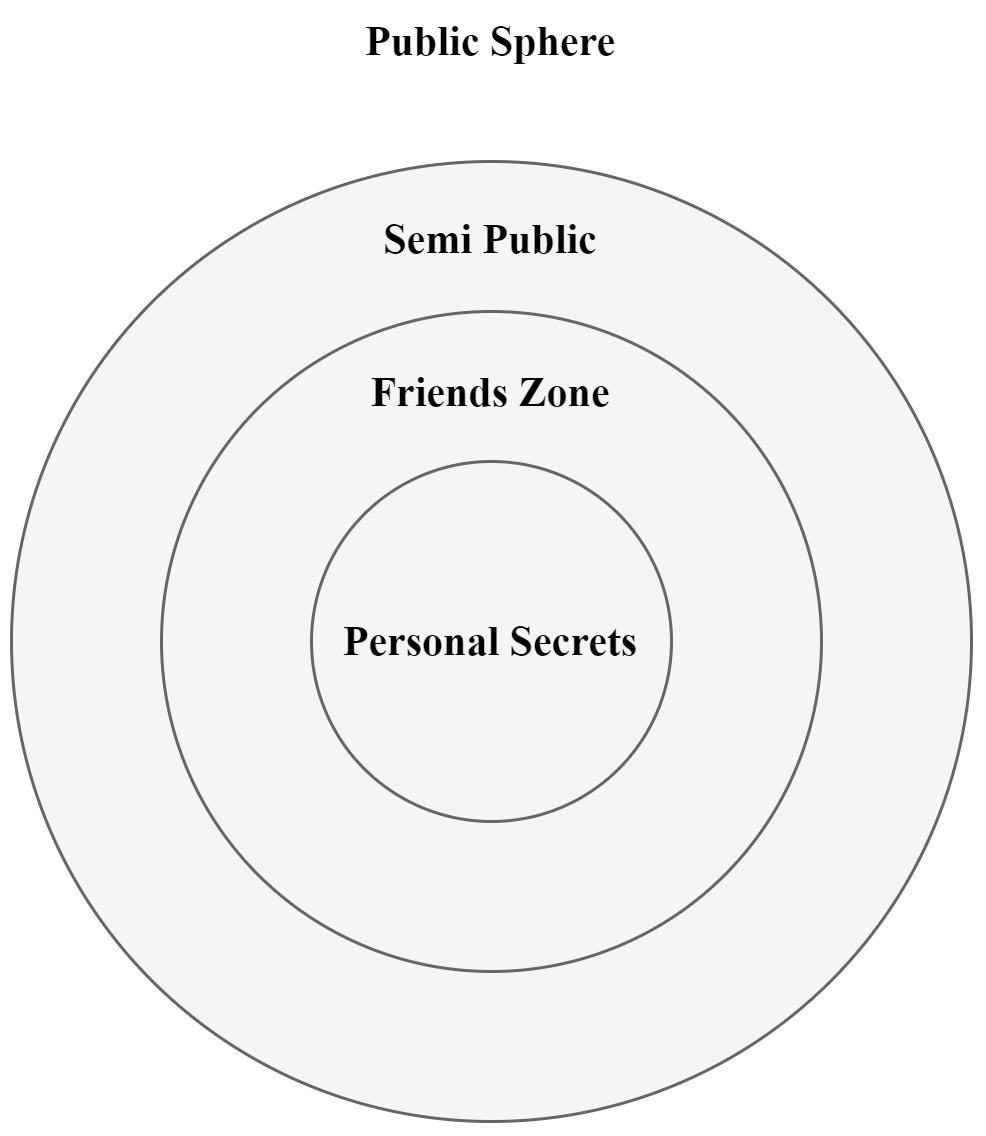
\includegraphics[width=0.8\linewidth]{img/spheres.png}
	\end{center}
\end{minipage}

\vspace{1em}
This means that any editing of personal data is \textbf{nota bene illegal}. Unless it is justified by the consent of the person whose rights are infringed or by law or by an overriding private or public interest.

\subsubsection{Legal Bases}
\begin{itemize}[label=-]
	\item Swiss Constituion Art 13
	\item Swiss Federal Act on Data Protection
	\item Ordinance to FADP (Verordnung zum Bundesgesetz über den Datenschutz, VDSG)
	\item EU-GDPR (General Data Protection Regulation - DSGVO)
\end{itemize}

\subsection{Changes in the New Data Protection Law (eDSG)}

\begin{itemize}[label=-]
	\item Only for natural entities (Art 2 eDSG)
	\item Extension of the territorial validity, abroad also (Art 2a eDSG)
	\item Naming a representative in Switzerland (Art 12 eDSG)
	\item Extention of Profiling (Art 4 lit f eDSG)
	\item Data Protection Consultant (Art 9 eDSG)
	\item List of processing activities (Art 11 eDSG)
	\item Data protection impact assessment (Art 20 eDSG)
	\item Reporting data security breaches (Art 22 eDSG)
	\item Legal claim for deletion of personal data (Art 28 Abs 2 lit c eDSG)
	\item Fines of up to 250'000 CHF are imposed on private persons who deliberately… (Art 55 eDSG)
\end{itemize}

\subsection{Area of Application Art 2 DSG}
\begin{enumerate}[label=\arabic*]
	\item This Act applies to the processing of data pertaining to natural persons and legal persons by:
	\begin{enumerate}[label=\alph*.]
		\item \textbf{private persons};
		\item federal bodies.
	\end{enumerate}
	\item \textbf{It does not apply to}:
	\begin{enumerate}[label=\alph*.]
		\item personal data that is \textbf{processed by a natural person exclusively for personal use and which is not disclosed to outsiders};
		\item deliberations of the Federal Assembly and in parliamentary committees;
		\item pending civil proceedings, criminal proceedings, international mutual assistance proceedings and proceedings under constitutional or under administrative law, with the exception of administrative proceedings of first instance;
		\item public registers based on private law;
		\item personal data processed by the International Committee of the Red Cross.
	\end{enumerate}
\end{enumerate}

\subsection{Terms and Definitions Art 3 DSG}
\begin{itemize}[label=]
	\item The following definitions apply:
	\begin{enumerate}[label=\alph*.]
		\item \textbf{personal data (data)}: all information relating to an identified or identifiable person;
		\item \textbf{data subjects}: natural or legal persons whose data is processed;
		\item \textbf{sensitive personal data}: data on:
		\begin{enumerate}[label=\arabic*.]
			\item religious, ideological, political or trade union-related views or activities,
			\item health, the intimate sphere or the racial origin,
			\item social security measures,
			\item administrative or criminal proceedings and sanctions;
		\end{enumerate}
		\item \textbf{personality profile}: a collection of data that permits an assessment of essential characteristics of the personality of a natural person;
		\item \textbf{processing}: any operation with personal data, irrespective of the means applied and the procedure, and in particular the collection, storage, use, revision, disclosure, archiving or destruction of data;
		\item \textbf{disclosure}: making personal data accessible, for example by permitting access, transmission or publication;
		\item \textbf{data file}: any set of personal data that is structured in such a way that the data is accessible by data subject;
		\item \textbf{federal bodies}: federal authorities and services as well as persons who are entrusted with federal public tasks;
		\item \textbf{controller of the data file}: private persons or federal bodies that decide on the purpose and content of a data file;
	\end{enumerate}
\end{itemize}

\subsection{Principles Art 4 DSG}
\begin{enumerate}[label=\arabic*]
	\item Personal data may only be processed \underline{lawfully}.
	\item Its processing must be carried out \underline{in good faith} and \underline{must be proportionate}.
	\item Personal data may only be processed \underline{for the purpose indicated at the time of collection}, that is evident from the circumstances, or that is provided for by law.
	\item The collection of personal data and in particular the purpose of its processing \underline{must be evident} to the data subject.
	\item If the consent of the data subject is required for the processing of personal data, such consent \underline{is valid only if given voluntarily} on the provision of adequate information. Additionally, consent must be given \underline{expressly} in the case of processing of sensitive personal data or personality profiles.
\end{enumerate}

\subsection{Accuracy of Personal Data Art 5 DSG}
\begin{enumerate}[label=\arabic*]
	\item Anyone who processes personal data \textbf{must make certain that it is correct}. He must take all reasonable measures to ensure that data that is incorrect or incomplete in view of the purpose of its collection is either \textbf{corrected or destroyed}. 
	\item \textbf{Any data subject may request that incorrect data be corrected}.
\end{enumerate}

\subsection{Cross-Border Disclosure Art 6 DSG}
\begin{enumerate}[label=\arabic*]
	\item Personal data \textbf{may not be disclosed abroad} if the privacy of the data subjects \textbf{would be seriously endangered thereby}, in particular due to the absence of legislation that guarantees adequate protection.
	\item In the absence of legislation that guarantees adequate protection, personal data may be disclosed abroad only if: ...
\end{enumerate}

\subsection{Accuracy of Personal Data Art 7 DSG}
\begin{enumerate}[label=\arabic*]
	\item Personal data must be protected against \textbf{unauthorised processing} through \textbf{adequate technical and organisational measures}.
	\item The Federal Council issues detailed provisions on the minimum standards for data security.
\end{enumerate}

\subsection{Right to Information Art 8 DSG}
\begin{enumerate}[label=\arabic*]
	\item Any person may request information from the controller of a data file as to whether data concerning them is being processed.
	\item The controller of a data file \textbf{must notify the data subject}:
	\begin{enumerate}[label=\alph*.]
		\item \textbf{of all available data} concerning the subject in the data file, including the available information on the \textbf{source of the data};
		\item \textbf{the purpose of} and if applicable \textbf{the legal basis} for the processing as well as the \textbf{categories of the personal data} processed, the other parties involved with the file and \textbf{the data recipient}.
	\end{enumerate}
	\item The controller of a data file may arrange for data on the health of the data subject to be communicated by a doctor designated by the subject.
	\item If the controller of a data file has personal data processed by a third party, \textbf{the controller remains under an obligation to provide information}. The third party is under an obligation to provide information if he does not disclose the identity of the controller or if the controller is not domiciled in Switzerland.
	\item The information must normally be provided in \textbf{writing, in the form of a printout or a photocopy, and is free of charge}. The Federal Council regulates exceptions.
	\item \textbf{No one may waive the right to information in advance}.
\end{enumerate}

\subsection{Right to be Informed}
\begin{itemize}
	\item \textbf{All judicious persons} are authorised
	\item An \textbf{owner of data collection} is legally obligated
	\item There is \textbf{no} form of request
	\item The range is \textbf{all} of the personal information
	\item Deadline to inform the requester \textbf{in written form or upon consent per insight within 30 days generally}
	\item \textbf{Generally free of charge}
\end{itemize}

\subsection{Duty To Provide Information On The Collection Of Sensitive Personal Data And Personality Profiles Art 14 DSG}
\begin{enumerate}[label=\arabic*]
	\item The controller of the data file \textbf{is obliged to inform the data subject} of the collection \textbf{of sensitive personal data or personality profiles}; this duty to provide information also applies where the data is collected from third parties.
	\item The data subject must be notified as a minimum of the following:
	\begin{enumerate}[label=\alph*.]
		\item the \textbf{controller of the data file};
		\item the \textbf{purpose} of the processing;
		\item the \textbf{categories of data recipients} if a disclosure of data is planned.
	\end{enumerate}
\end{enumerate}

\subsection{Breach Of Obligations To Provide Information, To Register Or To Cooperate Art 34 DSG}

\begin{enumerate}[label=\arabic*]
	\item On complaint, \textbf{private persons are \underline{liable to a fine}} if they:
	\begin{enumerate}[label=\alph*.]
		\item breach their obligations under Articles 8–10 and 14, in that they \textbf{wilfully provide false or incomplete information}; or
		\item wilfully fail:
		\begin{enumerate}[label=\arabic*.]
			\item \textbf{to inform the data subject in accordance with Article 14} paragraph 1, or
			\item \textbf{to provide information required under Article 14} paragraph 2.
		\end{enumerate}
	\end{enumerate}
	\item Private persons are \textbf{\underline{liable to a fine} if they wilfully}:
		\begin{enumerate}[label=\alph*.]
			\item \textbf{fail to provide information} in accordance with Article 6 paragraph 3 or to declare files in accordance with Article11a or who in doing so wilfully provide false information; or
			\item \textbf{provide the Commissioner with false information} in the course of a case investigation (Art 29) or who refuse to cooperate.
	\end{enumerate}
\end{enumerate}

\subsection{Breach Of Professional Confidentiality Art 35 DSG}
\begin{enumerate}[label=\arabic*]
	\item Anyone who without authorisation \textbf{wilfully discloses confidential, sensitive personal data or personality profiles} that have come to their knowledge in course of their professional activities where such activities require the knowledge of such data, \textbf{on complaint, liable to a fine}.
\end{enumerate}

\subsection{Data Processing by Third Parties Art 10a DSG}
\begin{enumerate}[label=\arabic*]
	\item The processing of personal data may be assigned to third parties by agreement of by law if:
	\begin{enumerate}[label=\alph*.]
		\item the data is processed \textbf{only in the manner permitted for the instructing party itself}; and
		\item \textbf{it is not prohibited by a statutory or contractual duty of confidentiality}.
		\begin{enumerate}[label=\arabic*.]
			\item The instructing party must in particular \textbf{ensure that the third party guarantees data security}.
			\item Third parties may claim the same justification as the instructing party.
		\end{enumerate}
	\end{enumerate}
\end{enumerate}

\subsection{Employment and Data Protection Art 328b OR}
"The employer may data about the employee \textbf{only} process as it concerns \textbf{his qualification for the employment} or are \textbf{inevitable for the execution of the employment}. The regulations of the Swiss Data Protection Act are applicable."

\subsection{EU-Law Is Applicable for Swiss Companies}

\begin{itemize}
	\item EU-GDPR
	\item Directly applicable for all swiss companies if they address to customers in the EU  and are collecting personal data
\end{itemize}

\section{General Data Protection Regulation}
GDPR is directly applicable for Swiss companies if they
\begin{itemize}
	\item offer products and services in the EU/EWR and handle personal data for that purpose
	\item collect and exploit the personal data of website visitors from the EU
	\item send regular newsletter to recipients in the EU
	\item handle personal data by order of or as a concern or part of a company domiciled in the EU
\end{itemize}
EU supervisory authorities have the power to conduct inspections, to request relevant information, to give orders and, in cases of severe disregard of the GDPR, to levy fines up to €10-20 Mio. or up to 2-4\% of the worldwide annual revenue.

\begin{center}
	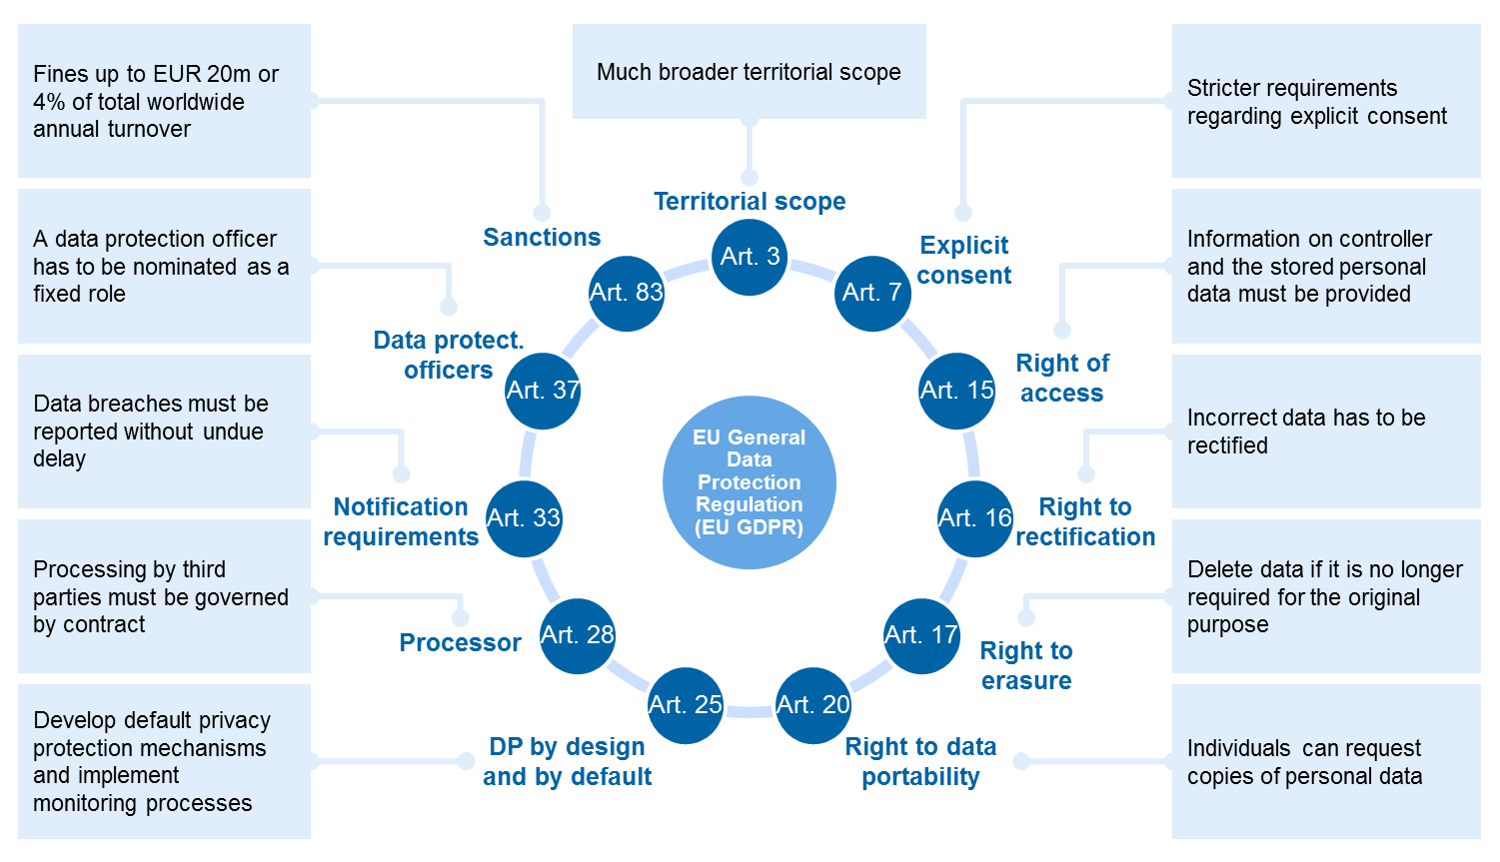
\includegraphics[width=0.9\linewidth]{img/gdpr_swiss_side}
\end{center}

\subsection{GDPR in Detail}
\begin{itemize}
	\item Augmenting of the peoples rights (Art 5/6 GDPR)
	\item Data storing only as long as it is necessary (storage limitation, Art 5 GDPR)
	\item Data protection by default by design (Art 25 GDPR)
	\item Big Data: Duty to do a Data protections impact assessment (Art 35 DSGVO)
	\item Duty to notify the supervisory authority of a personal data breach (Art 33 GDPR) and the data subject directly in cases of a high risk to the rights and freedoms of natural persons (Art 34 GDPR)
	\item Designation of a data protection officer (Art 37 GDPR). And if the requirements are met, a representative in the EU. (Art 27 Abs 1 DSGVO)
	\item When the processing is to be carried out on behalf of a controller: Only with sufficient guarantees, that is a contract (Art 28 Abs 1 GDPR)
	\item Right to data portability in a structured, commonly used and machine-readable format (Art 20 GDPR)
	\item Responsibility of the controller and duty to implement and document appropriate technical and organisational measures (Art 24 GDPR)
	\item No sub-sub-processing without written consent of the concerned party (Art 28 Abs 2 GDPR)
\end{itemize}

\subsection{Steps to Take}
\begin{center}
	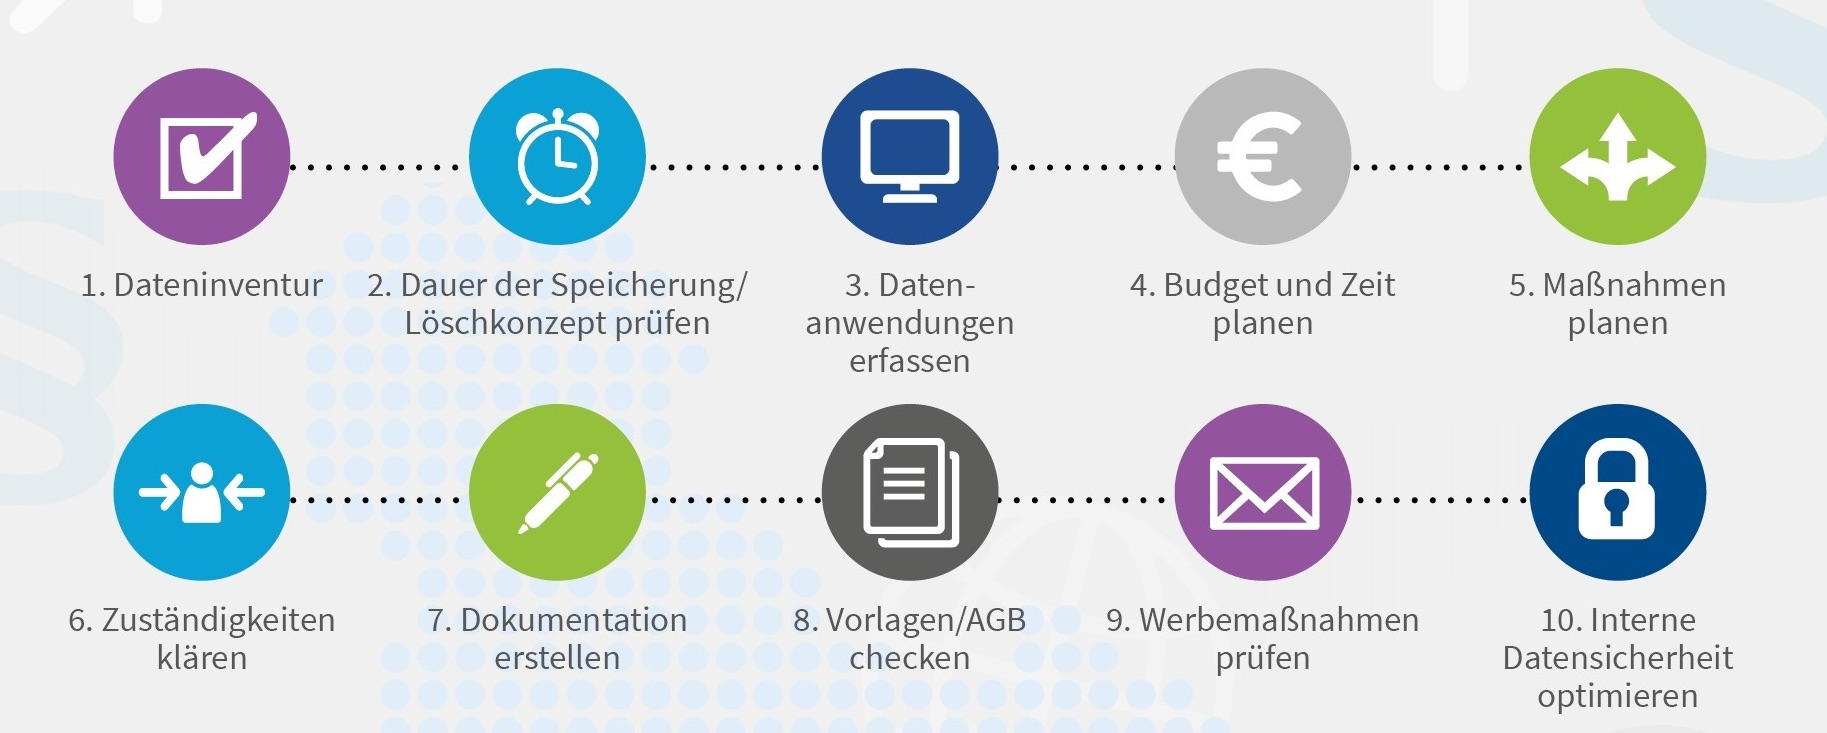
\includegraphics[width=\linewidth]{img/gdpr_step_by_step_plan}
\end{center}
The base of any data protection audit is to assess the actual situation.
\begin{itemize}[noitemsep]
	\item What personal data does exist?
	\item In what form and where?
	\item For what reason?
	\item Who is responsible?
	\item Who has access?
	\item How long will be the data stored?
	\item How is the data protected technically and organisationally?
	\item What are the estimated possible risks of a data breach and their consequences?
\end{itemize}
The GDPR requires to adapt existing contracts, declarations (terms of use) and proceedings. Companies have an augmented duty to document. Appointing and naming a Data Protection Officer and, for Swiss companies, a representative located in the EU is mandatory.

Implement Technical \& Operational Measures, do a thorough and detailed documentation of data systems and their organisation.

\subsection{Cookies}
The European Court of Justice (ECJ) decided that explicit consent is required for cookies. The website operator is obliged to provide evidence.

\section{Trademark and Designs}
Trademarks influence consumer decisions every day. A strong trademark creates an identity, builds trust, distinguishes from competitors, and facilitates communication between producers and consumers. Registering a trademark gives the \textbf{exclusive right to use a certain sign for specific goods and services}. The usage of the trademark by a third party may be granted through licensing. A trademark owner can \textbf{prevent others} from \textbf{using an identical or similar sign for the same or similar goods and services}.

The owner of a trademark work is entitled to the exclusive and sole right to determine for
\begin{enumerate}[noitemsep,nosep]
	\item What
	\item When
	\item How
	\item By whom
\end{enumerate}
his or her trademark may be used.

\subsection{Special Type of Trademarks}
\begin{enumerate}
	\item Trademarks that have acquired distinctiveness through use\\
	Coca Cola, Virgin
	\item Trademarks that have become generic through use\\
	Trademarks can become designations for entire product classes through years of market presence and therefore lose their protective status, for example Xerox for printers
	\item Famous Trademarks
	\item Indication of Source\\
	Indications of source do not differentiate certain goods or services from each other by the manufacturer of the product as trademarks do, but by their geographical origin.
	
	If a sign contains distinctive components alongside a direct indication of source, it can be registered in the trademark register. They may only be used for products which originate from the indicated geographical area.
\end{enumerate}
The name of a business is not automatically protected as a trademark, thus it should be registered
\begin{enumerate}[noitemsep, nosep]
	\item in the commercial register
	\item in the trademark register
	\item as a domain name, which can also be registered as trademarks
\end{enumerate}

\subsection{Grounds for Refusal}
\begin{enumerate}
	\item Signs belonging to the public domain must remain available to everyone and cannot be registered. This includes, for instance, single letters or numbers or abbreviations.A sign may also not be purely descriptive of a characteristic, quality, type or place of production.\\
	Apple may not be used for a type of fruit, but it can be registered for a company selling computers
	\item A trademark may not be misleading or deceptive regarding properties such as source or quality.
	\item A trademark may not be offensive to moral standards or against the law.
\end{enumerate}

A trademark is only protected for those classes of goods and services for which it has been registered. If a trademark is not used within 5 years of registration, it may lose it's protection.

\subsection{Duration of Trademark Protection}
A trademark is protected once it is registered for a term of 10 years. This protection may be renewed multiple times, so a trademark that is in use can be protected indefinitely.

\subsection{Principle of Territoriality}
Trademarks are only valid in the country where they are registered. A trademark registered in Switzerland is therefore only protected in Switzerland. Outside the country where a trademark is registered, there is no protection, others may freely use the trademark!

\begin{enumerate}
	\item Applying directly to the country concerned
	\item The Madrid System\\
	Under the Madrid System trademark protection granted under Swiss law may be extended to other states or organisations that have signed the Madrid contract.
	\item EU Community Trademark
\end{enumerate}
The IGE does not verify whether identical or similar IP rights such as trademarks, company or domain names already exist. Potential conflicts with rights of other people are thus not examined in the registration process.

Checks before registering a trademark:
\begin{enumerate}
	\item Ensure that the sign is distinctive
	\item Search trademark registries
	\item Search commercial registers and domain names
\end{enumerate}

\subsection{Opposition or Cancellation}
\begin{enumerate}
	\item Opposition proceedings\\
	With publication on the Swiss register, the three-month opposition period begins and owners of prior identical or similar trademarks can file opposition to that mark during this period.
	\item Cancellation proceedings\\
	Any person is allowed to request the cancellation of a trademark registration on the grounds of non-use.
\end{enumerate}

\subsection{Design}
In the legal sense, design is understood to be the exterior form of a product or parts of it. It can be either two-dimensional or three-dimensional. Its form is characterised by the arrangement of lines, contours, colours and surfaces or by the material used.

Design appeals to our senses, evokes feelings, creates identity and distinguishes itself. This is why design has become one of the most crucial market factors and why counterfeiting is subsequently a frequent occurrence in this field.

Owners of a design right can prevent others from manufacturing, storing, offering, putting on the market, importing, exporting or transporting of such products as well as  being in possession of them.

Criteria for protection:
\begin{itemize}[label=-,noitemsep]
	\item The design is new, meaning no other identical or similar design has been published before application;
	\item The design is sufficiently different from existing designs in major characteristics.
\end{itemize}

A registered design is protected for a period of 5 years, this term can be extended by 5 years until a maximum of 25 years.

\section{Compliance and Records Management}
\begin{definition}
	The term compliance describes the ability to act according to an order, set of rules or request.\\
	Compliance operates at two levels:
	\begin{enumerate}
		\item \textbf{Compliance with external rules} that are imposed upon an organisation as a whole
		\item \textbf{Compliance with internal systems of control} that are imposed to achieve compliance with the external rule
	\end{enumerate}
\end{definition}
Corporate Governance is a concept that covers a number of different aspects about the way in which an organisation is managed, directed and governed.

It can be described as a set of relationships between a company’s management, board, shareholders, and other stakeholders, which provides the structure through which the objectives of the company are set. Furthermore it provides the means of attaining and monitoring performance against those objectives.
\subsection{Key Functions of Compliance}
\begin{enumerate}
	\item \textbf{Identification}\\
	To identify the risks that an organisation faces
	\item \textbf{Prevention}\\
	To design and implement controls to protect an organisation from those risks
	\item \textbf{Monitoring and Detection}\\
	To monitor and report on the effectiveness of those controls
	\item \textbf{Resolution}\\
	To resolve compliance difficulties as they occur
	\item \textbf{Advisory}\\
	To advise the business on rules and controls
\end{enumerate}

\subsection{Risk Management}
To know and handle your risks, as it is dangerous to not know them. Assess the risks the organisation may face professionally, and define limits. Control the risk prevention periodically. Most of the time, not all risks can be averted, so have a constant awareness but flexible risk handling.

\subsection{Records Management}
\begin{minipage}{0.6\linewidth}
	\textbf{Life cycle of information}
	\begin{enumerate}
		\item create
		\item record
		\item use
		\item share
		\item archive
		\item delete
	\end{enumerate}
\end{minipage}
\begin{minipage}{0.4\linewidth}
	\centering
	
\includegraphics[width=0.8\linewidth]{img/information_life_cycle.png}
\end{minipage}

\vspace{1em}
\noindent
The most important task is to categorise each document or record into
\begin{itemize}
	\item \textbf{Non-essential}
	\item \textbf{Useful}
	\item \textbf{Important}
	\item \textbf{Vital}
\end{itemize}
These categories have to be treated differently, otherwise they lose their usefulness. Different categories have different safekeeping periods (possibly imposed by compliance):

5 or 10 years from the beginning of the new fiscal year.

\subsection{Criminal Liability}
\subsubsection{Art 166 StGB}
"Any debtor who fails to comply with a statutory obligation to which he is subject to keep and preserve business accounts or draw up a balance sheet, with the result that his financial position is not or not fully ascertainable, is liable, if bankruptcy proceedings are commenced against him or a certificate of unsatisfied claims has been issued in his respect following a seizure of assets in accordance with Article 43 DEBA (SchKG), to a custodial sentence not exceeding three years or to a monetary penalty."

\subsubsection{Art 325 StGB}
"Any person who wilfully or through negligence fails to comply with the statutory duty to keep proper accounts or to preserve accounts, business correspondence and business telegrams, any person who wilfully or through negligence fails to comply with the statutory duty to preserve accounts, business correspondence and business telegrams, is liable to a fine."

\subsection{Responsibility of the Board of Directors Art 754 OR}
\begin{enumerate}[label=\arabic* ]
	\item The members of the board of directors and all persons engaged in the business management or liquidation of the company are liable both to the company and to the individual shareholders and creditors for any losses or damage arising from any intentional or negligent breach of their duties.
	\item A person who, as authorised, delegates the performance of a task to another governing officer is liable for any losses caused by such officer unless he can prove that he acted with all due diligence when selecting, instructing and supervising him.
\end{enumerate}

\subsection{Keeping and Retaining Accounting Records Art 958f OR}
\begin{enumerate}[label=\arabic* ]
	\item The accounting records and the accounting vouchers together with the annual report and the audit report must be retained \textbf{for ten years}. The \textbf{retention period begins on expiry of the financial year}.
	\item The annual report and the audit report must be retained in a written form and signed.
	\item The accounting records and the accounting vouchers may be retained on paper, electronically or in a comparable manner, provided that correspondence with the underlying business transactions and circumstances is guaranteed thereby and provided they can be made readable again at any time.
	\item The Federal Council shall issue regulations on the accounting records that must be kept, the principles for keeping and retaining them and on the information carriers that may be used.
\end{enumerate}

\subsection{Decree Over the Keeping and Archiving of Business Records Art 2 GEBÜV}
\begin{enumerate}[label=\arabic* ,start=2]
	\item If the books of account are kept and preserved electronically or in a comparable manner and the accounting documents are recorded and preserved electronically or in a comparable manner, the \textbf{principles of proper data processing must be observed}.
\end{enumerate}

\subsection{Integrity (Authenticity and Immutability) Art 3 GEBÜV}
The accounts must be kept and retained in such a way and the supporting documents must be recorded and retained in such a way that they cannot be altered without it being possible to establish that they have been altered.

\subsection{Documentation Duties Art 4 GEBÜV}
\begin{enumerate}[label=\arabic* ]
	\item Depending on the nature and extent of the business, the organisation, responsibilities, processes and procedures and infrastructure (machinery and programmes) used in the maintenance and safekeeping of accounts shall be documented in work instructions in such a way that the accounts and accounting records can be understood.
	\item Work instructions shall be updated and retained in accordance with the same principles and for the same length of time as the books of account kept thereafter.
\end{enumerate}

\section{Patent Law and Design Law}
A patent is a vital element for successful commercialisation, as it gives the absolute right to use the patent. Patent protection constitutes an essential incentive to innovate, and indeed much innovation would not take place without patents. The publication of patent applications is mandatory 18 months after they are filed and provides access for the public to the latest technical developments.

The patent system serves as an effective transmission belt for the spread of knowledge and information on state-of-the-art technologies. The main purpose is the promotion of scientific research and innovation.
\begin{enumerate}
	\item Protection shall be a guarantee and an incentive for investments in research and development
	\item Protection of the invention is granted
	\begin{enumerate}
		\item only in exchange for the disclosure of the invention
		\item only for a limited period of time
	\end{enumerate}
	\item At the same time third parties are incentivised to search for new solutions
\end{enumerate}

As an absolute right, a patent confers on its holder the right to prohibit others from commercially using the invention.

A patent as such does not confer on its owner the right to use an invention as the patent law does not govern whether and under which conditions an invention may be used. Rather, this is the subject matter of other laws, which may provide for restrictions.

\subsection{Patentability}
Before an invention can be patented it must be
\begin{enumerate}
	\item New
	\item Involve an inventive step
	\item Susceptible of industrial application
	\item Not expressly excluded from patent protection
\end{enumerate}

\begin{itemize}[leftmargin=*, labelindent=4cm, labelsep=1cm]
	\item[\textbf{Formal Requirements}] Registration
	\item[\textbf{Exclusive Right}] User for commercial purposes
	\item[\textbf{Term of protection}] 20 years from filing date
\end{itemize}

\subsubsection{Protection Requirements}
\begin{enumerate}
	\item \textbf{Industrial application}\\
	The invention must be manufacturable or applicable in some commercial sector
	\item \textbf{Novelty}\\
	An invention is only novel when its technologies are not already part of the state of the art.
	\item \textbf{Non-obvious}\\
	The solution to a problem is not obvious if it involves an inventive step which is non-obvious to a person with the necessary skill and knowledge
\end{enumerate}

\subsubsection{Exclusions}
The following are not regarded as inventions (Art 52 Para 2 EPC):
\begin{enumerate}
	\item \textbf{discoveries}, scientific \textbf{theories} and mathematical \textbf{methods}
	\item \textbf{aesthetic} creations
	\item \textbf{schemes, rules and methods} for performing mental acts, playing games or doing business and \textbf{programs for computer}
	\item presentations of information
\end{enumerate}
The \textbf{human body} as such, at all stages of its formation and development, including the embryo, or elements of the human body in their natural environment, \textbf{is not patentable} (Art 1a Para 1 PatA).\\
The following inventions are \textbf{not patentable} (Art 2 PatA):
\begin{enumerate}
	\item Inventions whose exploitation is contrary to \textbf{human dignity} or that disregard the integrity of living organisms or that are in any other way contrary to public policy or morality are not patentable. In particular:
	\begin{enumerate}
		\item processes for \textbf{cloning} human beings and the clones obtained thereby;
		\item processes for forming \textbf{hybrid organisms by using human germ / embryonic stem cells};
		\item the use of human \textbf{embryos} for non-medical purposes;
		\item processes for modifying the genetic identity of animals which are likely to cause them suffering
	\end{enumerate}
	\item \textbf{Diagnostic, therapies and surgery procedures} used for humans or animals
	\item Plant varieties, animal breeds, and other primarily \textbf{biological procedures for breeding plants or animals}
\end{enumerate}
An element of the human body \textbf{is} patentable as an invention if it is produced by means of a technical process, a beneficial technical effect is indicated and the further requirements as set out in Patents Act are fulfilled.

\subsection{Formal Requirements for Patent Application}
Any person who wishes to obtain a \textbf{patent for an invention in Switzerland} must file a patent application with the Swiss Federal Institute of Intellectual Property (Art 49 para 1 PatA).
\begin{enumerate}
	\item A request for grant of a patent
	\item A description of the invention
	\item The patent claims
	\item Drawings on the description / patent claims
	\item An abstract
	\item The name of the inventor (Art 5 PatA)
	\item Priority claims (Art 17 ss PatA)
\end{enumerate}
Patents know the concept of joint inventors.

\subsection{Rights to a Patent in Employment}
\label{ss:RightEmployment}
\begin{enumerate}
	\item If the \textbf{employment contract} deals with this issue
	\item If the employment contract does not cover this issue, then article 332 of the Swiss Obligation Code applies: inventions (and designs) belong to the employer if they are made in \textbf{fulfillment of contractual obligations and in the course of his work}.
	\item Inventions (and designs) created \textbf{during regular work time} but \textbf{not under the contractual obligations} must be offered to the employer. Then the employer can decide whether he wants to obtain the invention (or design) in question.
\end{enumerate}

\subsection{Protection Abroad}
\begin{itemize}
	\item Filing directly in each country of interest
	\item Filing a European application
	\item Filling an internaional application
\end{itemize}
But, there is only a twelve month protection period from filing. During this period, you can file for a patent abroad and claim the date of your first application, so that novelty and non-obviousness will be assessed with regard to the date of first application.

\subsection{Strategies for Protecting an Invention}
\begin{enumerate}
	\item Protect the invention with a patent
	\item Publish an invention  without patenting it, thereby preventing anyone else from filing a patent
	\item Contractually bind the designers under a Trade Secret with confidentiality agreements
\end{enumerate}

\subsection{Patent Databases}
Patent databases contain a huge amount of information about technological developments for products and processes, which can be used to avoid developing a known solution.

\subsubsection{Patent Pending}
Once a patent application has been filed, an inventor can mark the invention as "patent pending". This gives no legal protection, but most companies do not want to risk a patent lawsuit in the future and respect the value of this designator.

\subsection{Copyright and Software}
Copyright and patent protection complement each other
\begin{enumerate}
	\item Copyright protects creators against copying existing programs
	\item Patent law protects against the exploitation of underlying ideas in new programs
\end{enumerate}

\subsection{Design}
A design is the exterior form of a product. It can be two-dimensional or three-dimensional. Its form is characterised by the arrangement of lines, contours, colours and surfaces or by the material used.

Design appeals to our senses, evokes feelings, creates identity and distinguishes itself. Thus, it is a crucial market factor which has to be protected against counterfeiting. Owners of a design right can prevent others from manufacturing, storing, offering, putting on the market, importing, exporting or transiting of such products.

\subsubsection{Filing a Design}
Criteria for protection
\begin{enumerate}
	\item Novelty
	\item Sufficient difference to existing designs
\end{enumerate}
However, the IGE does not determine novelty or distinctiveness of a filing. Third parties may contest the design at any time by initiating court proceedings. A registered design is protected for an initial period of 5 years, and can be extended four times for a maximum duration of 25 years.

The rightsholder is determined the same as in patents in subsection \ref{ss:RightEmployment}.

\section{Contract Law}
The Swiss Code of Obligations — General provisions on conclusion of contracts performance and non-performance defines
\begin{enumerate}[nosep]
	\item Conclusion of the contract (How to reach consent: Mutual expression of intent)
	\item Form of contract
	\item Defects of consent: error, fraud, duress
	\item Representation: authorisation to act on someone else's behalf
	\item Performance of obligation (place, time, payment)
	\item Breach of contract: the consequences of non-performance on obligations
	\item Third parties
	\item Time limits
\end{enumerate}

\subsubsection{Swiss Code of Obligations (CO) Art 1}
\begin{enumerate}[label=\arabic* ]
	\item The conclusion of a contract requires a mutual expression of intent by the parties
	\item The expression of intent may be express or implied
\end{enumerate}
\begin{definition}
	A contract defines
	\begin{itemize}[noitemsep,label=]
		\item \textbf{Who}
		\item \textbf{What}
		\item \textbf{Where}
		\item \textbf{How}
		\item \textbf{When}
		\item \textbf{For how long}
		\item \textbf{For how much}
	\end{itemize}
\end{definition}

Everybody has the \textbf{freedom of contract}, which means that there must be an \textbf{offer and acceptance} with mutual \textbf{consent} over \textbf{essential terms}. As a rule a contract does not have to be in written form.

The legal impact is only in relation to the contracting parties. Contract creates rights and obligations between these. Any change to the contract must be mutually agreed. Enforcement only against the other contracting parties.

\subsection{Freedom of Contract Art 19 CO}
\begin{enumerate}[label=\arabic* ]
	\item The terms of a contract may be \textbf{freely determined} within the \textbf{limits of the law}.
	\item Clauses that deviate from those prescribed by law are admissible only where the law does not prescribe mandatory forms of wording or where deviation from the legally prescribed terms would \textbf{contravene public policy, morality or rights of personal privacy}.
\end{enumerate}

\subsection{Freedom of Contract Art 20 CO}
\begin{enumerate}[label=\arabic* ]
	\item A contract is \textbf{void} if its terms are \textbf{impossible, unlawful or immoral}.
	\item However, where the defect pertains only to certain terms of a contract, those terms alone are void unless there is cause to assume that the contract would not have been concluded without them.
\end{enumerate}

\begin{enumerate}
	\item \textbf{Freedom to conclude or not conclude a contract}
	\item \textbf{Freedom to choose the contractual partner}
	\item \textbf{Freedom to alter or terminate a contract}
	\item \textbf{Freedom of form}\\
	A contract may be concluded verbally or even by a consenting behavior
	\item \textbf{Freedom of type}\\
	Freedom to conclude any kind of contract regardless of whether or not it is
	one of the individual types of contracts regulated by the Code of Obligations
	\item \textbf{Freedom to define the content of the contract}
\end{enumerate}
The Swiss Code of Obligations contains only few mandatory provisions. These aim at protecting one of the parties that the legislator deems to be the weaker one in the relationship (for example in employment, rent or lease contracts).

\subsection{Freedom to conclude a contract}
\subsubsection{Art 11 Civil Code}
Every person has \textbf{legal capacity}. Accordingly, within the limits of the law, every person has the same capacity to have rights and obligations.

\subsubsection{Art 12 Civil Code}
A person who has \textbf{capacity to act} has the \textbf{capacity to create rights and obligations} through his actions.

\subsubsection{Art 13 Civil Code}
A person who \textbf{is of age} and is \textbf{capable of judgement} has the capacity to act.

\subsubsection{Art 14 Civil Code}
A person is of age if he or she has reached the age of \textbf{18}.

\subsubsection{Art 16 Civil Code}
A person is \textbf{capable of judgement} within the meaning of the law if he or she does not lack the \textbf{capacity to act rationally} by virtue of being under age or because of a mental disability, mental disorder, intoxication or similar circumstances.

\subsubsection{Minors}
Minors and persons capable of judgement but lacking the capacity to act may only enter into a contract with the \textbf{consent of their legal representative}. Without representation they may only \textbf{accept advantages that are free of charge} or \textbf{carry out minor everyday transaction}.

\subsection{Written Form}
A contract may be concluded \textbf{verbally} or even without using words but by giving tacit approval through \textbf{consenting behaviour}. Written form is mandated if one or both parties require protection, as such contracts may have a great impact on their lives.

Most parties choose the written form voluntarily in order to have clarity and proof, this written form is acquired by the \textbf{personal signature}.

\subsection{Defects in the conclusion of a contract}
\begin{enumerate}[label=\arabic* ]
	\item If the diverging interpretations of both parties are equally admissible, there is no consent but rather \textbf{dissent} and, therefore, \textbf{no contract} has ever come into legal existence.
	\item The Code of Obligations establishes three cases where a defect in the conclusion of a contract result in the contract being \textbf{null and void from the outset}
	\begin{enumerate}
		\item the contractual terms are impossible from the onset (Art 20 I)
		\item the contractual terms are unlawful or immoral (Art 20 I)
		\item a prescribed formal requirement has not been fulfilled (Art 11)
	\end{enumerate}
\end{enumerate}

\begin{center}
	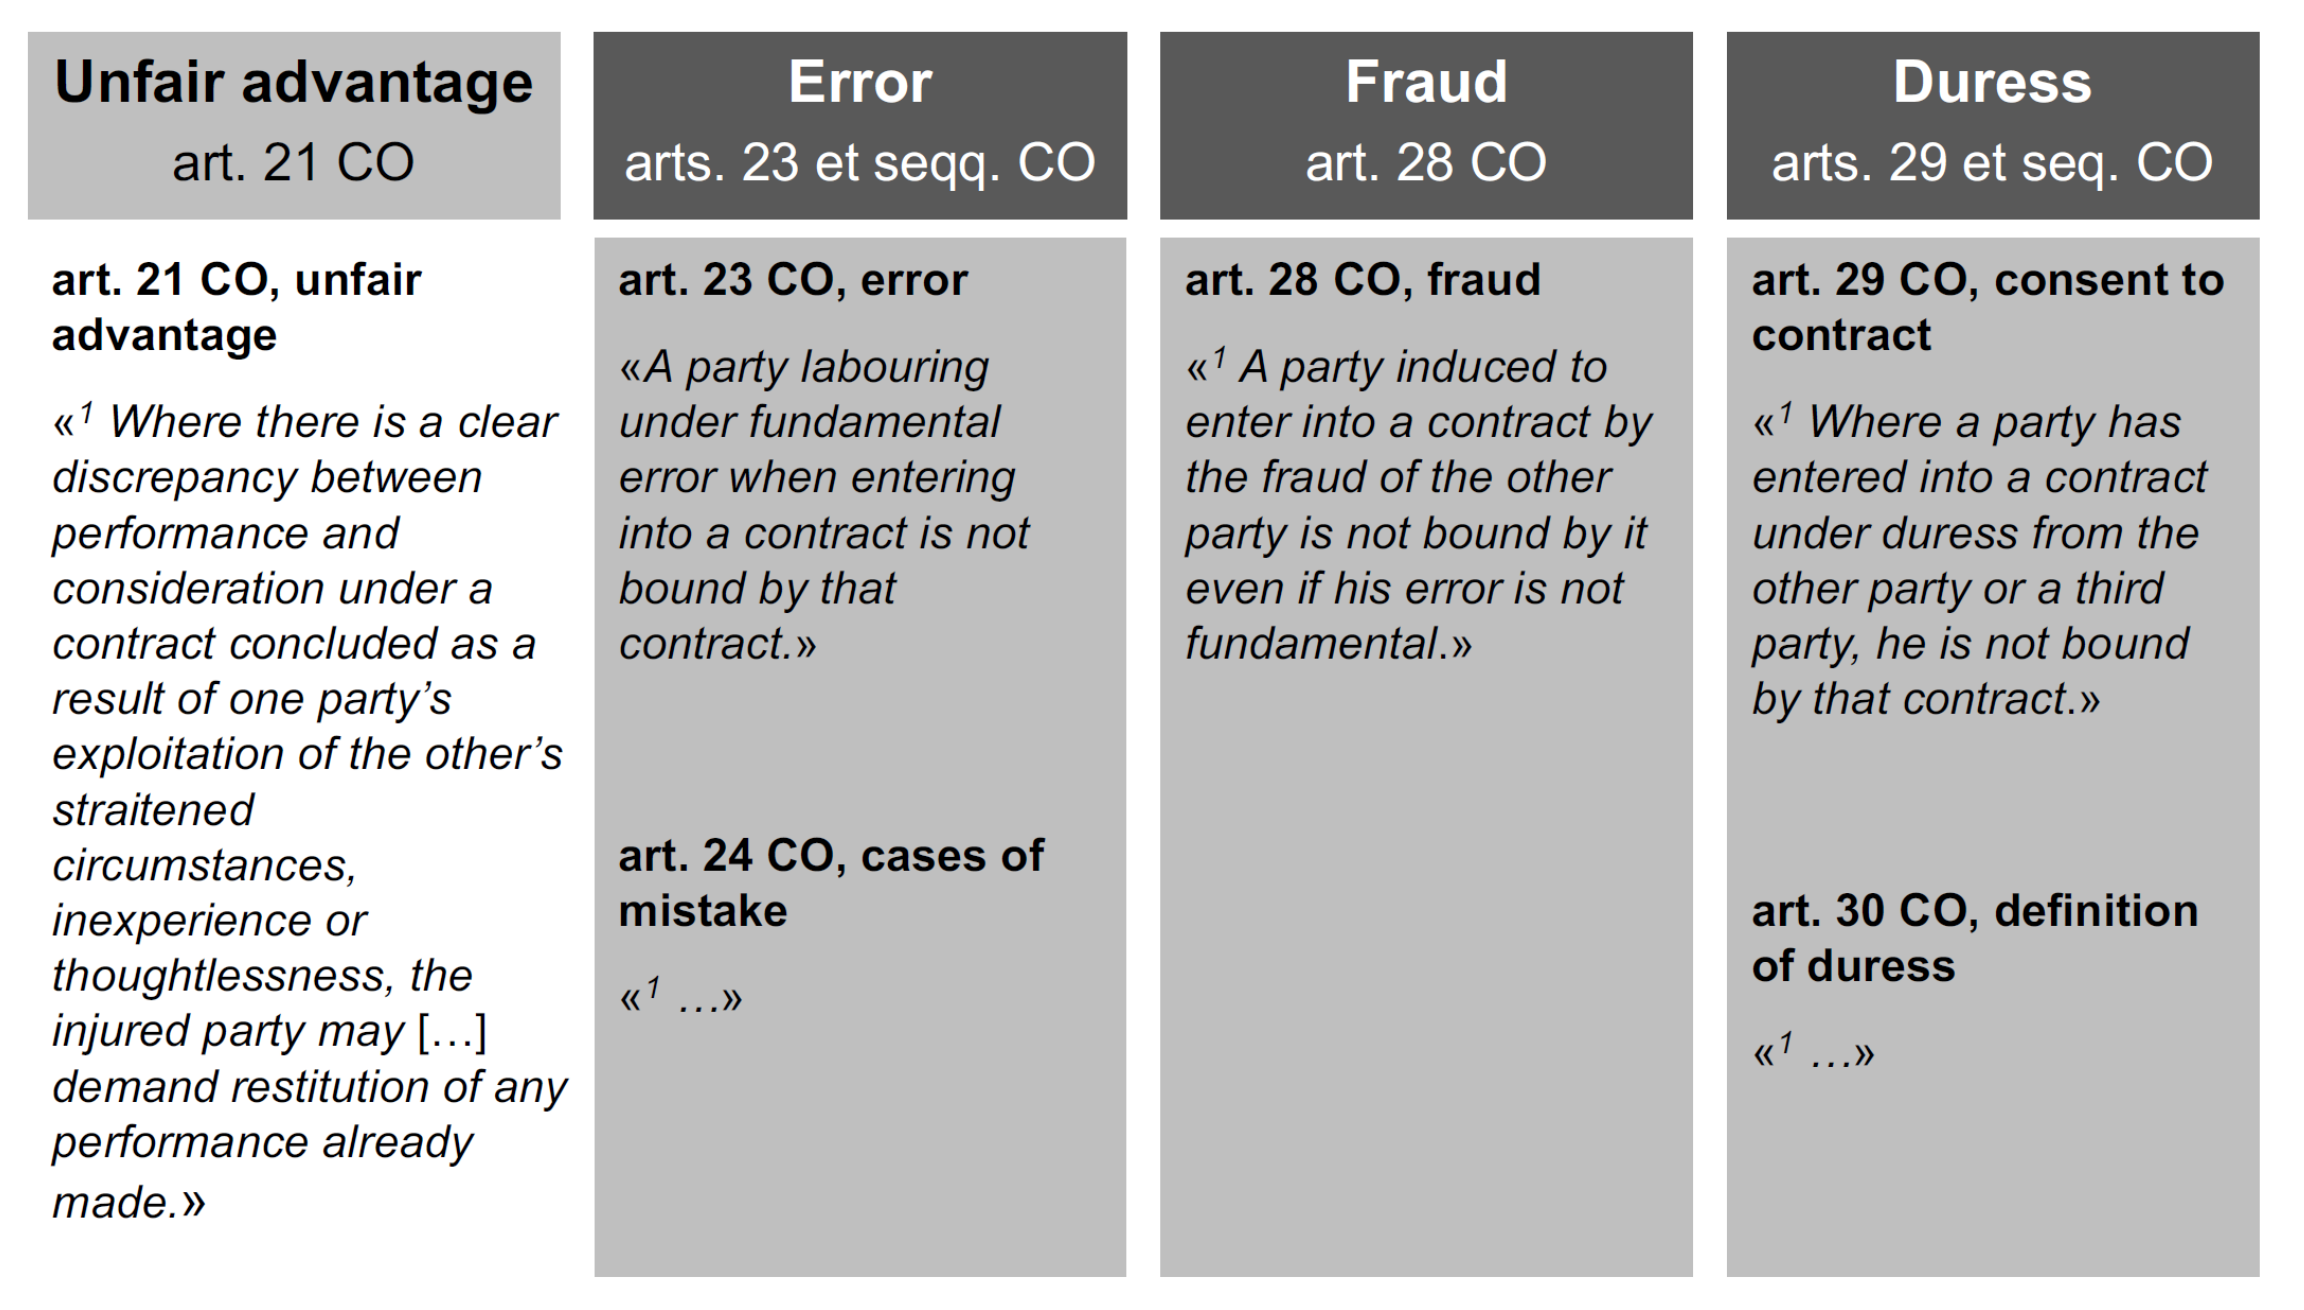
\includegraphics[width=0.8\linewidth]{img/defects_contract}
\end{center}

\subsection{Interpretation of a Contract}
\begin{enumerate}
	\item The interpretation of a contract shall be mainly led by the \textbf{principle of will}
	\item Only where there is doubt about the common intention of the parties does the \textbf{principle of trust} become relevant. The basis of the principle is thus largely seen as stemming from the \textbf{duty to act in good faith}.
\end{enumerate}

\subsection{Performance and Non-Performance of Obligations}
The contract defines type, scope and time of service provision. While the \textbf{warranties} determine the liability for defects and for any resulting damages.

\subsubsection{Damages Art 97 CO}
An obligor who fails to fulfill an obligation completely or as required is liable for the \textbf{resulting loss or damage} unless he can prove that he was not at fault.

\subsubsection{Damages Art 99 CO}
The obligor is generally liable for \textbf{any fault attributable to him}.

\subsubsection{Damages Art 100 CO}
Any agreement purporting to \textbf{exclude liability} for \textbf{unlawful intent or gross negligence} in advance is void.

\subsubsection{Prerequisites for Liability for Damages}
Burden of proof is on the party claiming damages
\begin{enumerate}
	\item damage
	\item breach of contractual duty
	\item causality between the damage and the breach
	\item \textbf{fault is attributable to the obligor}
\end{enumerate}
The contractual penalty must be contractually agreed and is due in the event of an infringement of a contractual duty.

If a \textbf{damage} has occurred, damages are to be paid if the damages exceed the amount of the contractual penalty. The parties may agree in the contract that contractual penalties are due \textbf{in addition to damages}.
If the amount of the contractual penalty is extremely high, a court may reduce them.

\subsubsection{Obligations in Tort Art 41 CO}
Any person who \textbf{unlawfully} causes \textbf{loss or damage} to another, whether \textbf{willfully or negligently}, is obliged to provide compensation.

\subsubsection{Obligations in Tort Art 49 CO}
\begin{enumerate}[label=\arabic* ]
	\item Any person whose personality rights are unlawfully infringed is entitled to a sum of money by way of satisfaction provided this is justified by the seriousness of the infringement and no other amends have been made.
	\item The court may order that satisfaction be provided in another manner instead of or in addition to monetary compensation.
\end{enumerate}

\subsubsection{Prerequisites for Liability for Tort}
The burden of proof is on the party claiming damages
\begin{enumerate}
	\item damage
	\item illegality
	\item adequate causal connection between the damage and actions of the defendant
	\item \textbf{fault is attributable to the defendant}
\end{enumerate}
Tort means there is no contract, but a party is held liable for damages.

\subsection{Time Limits}
\begin{tabularx}{\linewidth}{l c X}
	\hline
	\textbf{Contract or Tort} & \textbf{Article in CO} & \textbf{Time Limit}\\
	\hline
	Contract Law in general & 127 CO & After 10 years unless otherwise provided by federal civil law.\\
	Recurring contractual duties & 128 CO & After 5 years for: rent / lease and all other periodic payments; claims in connection with delivery of foodstuffs, payments for board and lodging and hotel expenses; claims in connection with work carried out by tradesmen, purchases of retail goods, medical treatment, professional services provided by attorneys / lawyers, work performed by employees for their employers.\\
	Personal injury due to breach of contract & 128a CO & After 3 years for injury or death in breach of contract, in any event 20 years after the date on which the harmful conduct took place.\\
	Tort & 60 CO & After 3 years from the date on which the person suffering damage became aware of the loss, damage or injury and of the identity of the person liable for it, but in any event 10 years after the date on which the harmful conduct took place, in cases of death or injury, 20 years
\end{tabularx}

\subsection{General Terms and Condition}
General Terms and Conditions are predefined contracts a provider or seller concludes with its customers. The aim is to gain efficiency and allocate risks. They apply whether they have been read or not, given they have been \textbf{accepted}. General Terms and Conditions provided \textbf{after acceptance} by customer \textbf{are not valid and do not apply}.

\subsubsection{Limitations}
If the terms and conditions are unusual, that is the consumer could not have expected them, they are unclear to the customer or if they create a considerable and unjustified disparity,

\subsection{Contracts codified in the Code of Obligations}
\begin{itemize}
	\item Purchase Contract
	\item Lease
	\item Loan
	\item Employment Contract
	\item Contract for Work and Services
	\item Services Contract
	\item Publishing Contract
	\item Commission Contract
	\item Guarantee
\end{itemize}
Contracts outside the Code of Obligations
\begin{itemize}
	\item Consumer Credit Act
	\item Product Liability Act
	\item Package Travel Act
\end{itemize}

\subsubsection{Purchase Contracts}
\textbf{Warranty}
\begin{itemize}
	\item Guaranteed features
	\item Defects that diminish value
	\item Reduce suitability for the intended use
	\item Maliciously concealed defects
\end{itemize}
The purchaser has the obligation to inspect the purchased goods as soon as practicable in the ordinary course of business, and the duty to give notice of defects immediately unless the defect were undetectable or defects occurred later or in the event of maliciously concealed defects (deception).

The purchaser has then the following options
\begin{enumerate}
	\item \textbf{Conversion}\\
	The purchase is reversed: the seller and purchase exchange the goods and the money paid (plus interest and costs incurred) back, unless the purchase has already resold or remodeled the goods, or the goods have perished
	\item \textbf{Reduction}\\
	The purchase contract is maintained but the seller has to compensate for the reduced value
	\item \textbf{Replacement}\\
	The purchase contract is maintained but the seller has to replace the defect goods with proper goods
\end{enumerate}
\begin{center}
	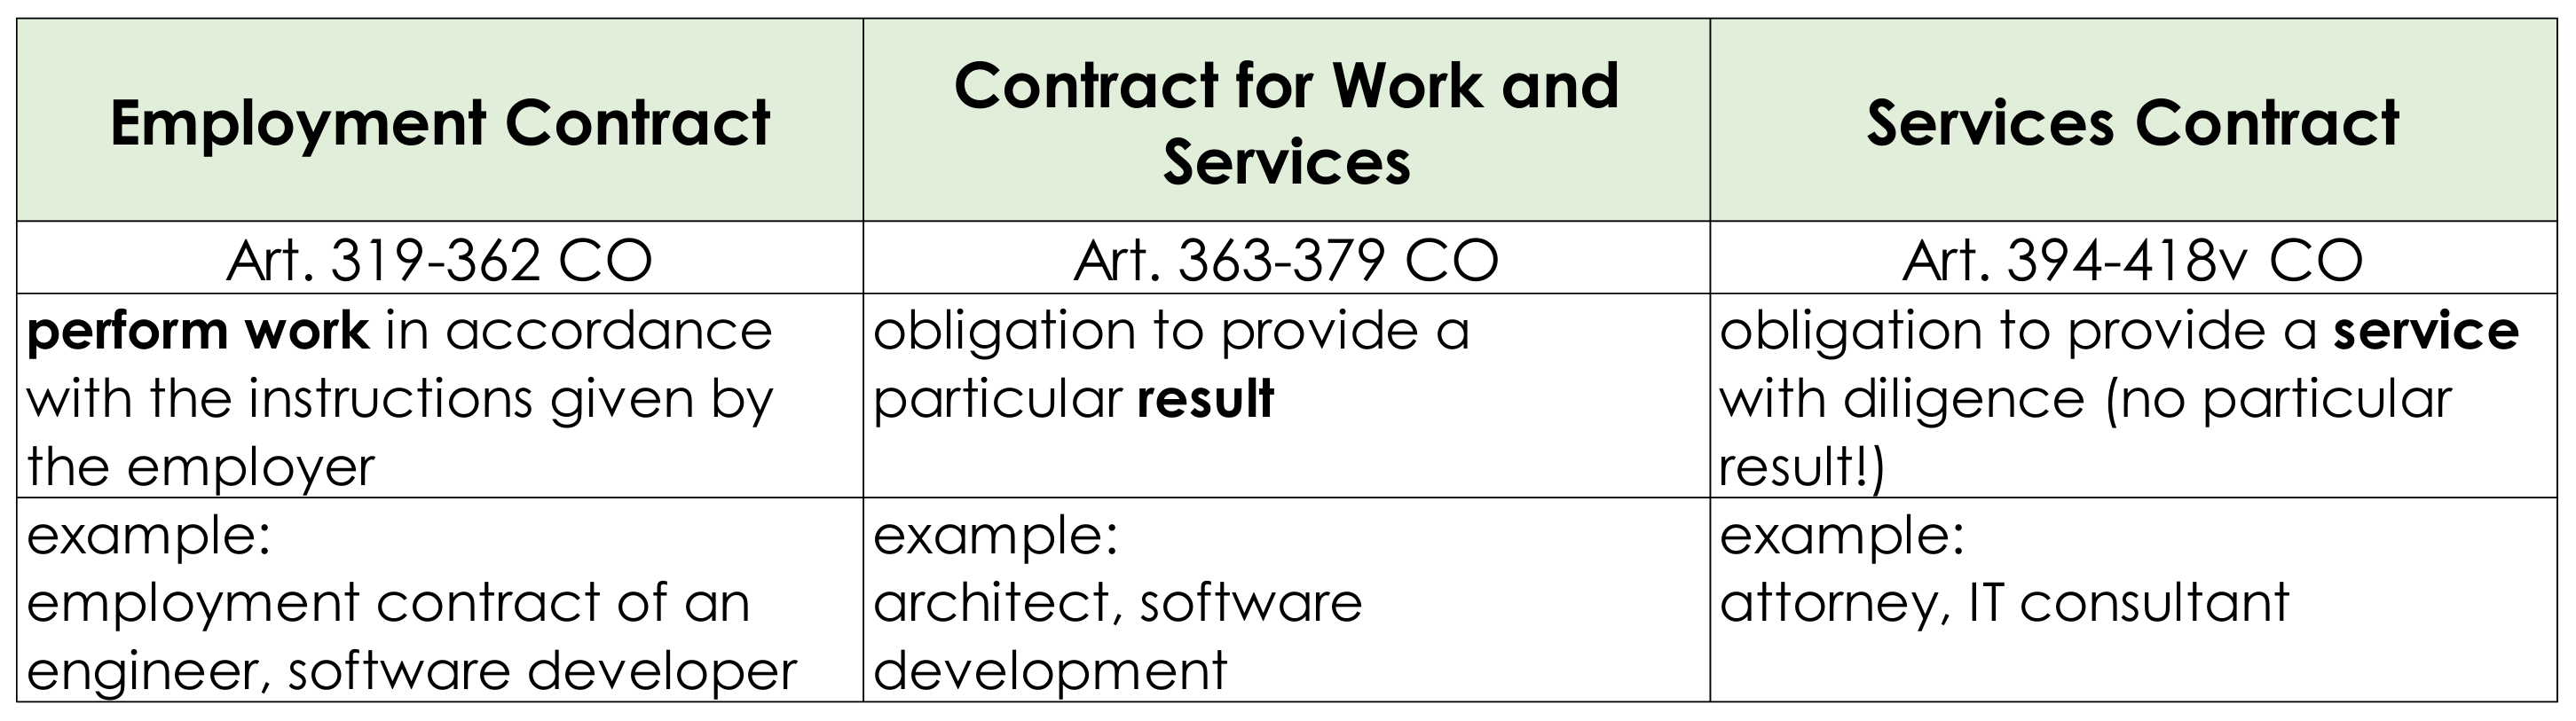
\includegraphics[width=0.9\linewidth]{img/type_contracts_work}
\end{center}

\subsection{Employment Contracts}
Employment contracts can be agreed for (1) a fixed term or (2) open-ended. Individual employment contracts are not subject to any formal requirements and may also be concluded by verbal agreement, with exception to apprenticeship contracts. If the employment contract does not contain a provision on the notice period the provisions of the Code of Obligations apply:
\begin{enumerate}
	\item 7 calendar days during the probation period
	\item 1 month during the first year of service
	\item 2 months from the second to the ninth year of service
	\item 3 months from the tenth year of service
\end{enumerate}
If the employment contract was not concluded for a fixed term, either party may terminate the contract at any time within the applicable notice period. Termination is only effective once the letter of termination has been received by the other party. The reason for the termination does not have to be stated.

Only for the termination with immediate effect does the terminating party need to provide reasons.

For open-ended employment contracts, the probation period is at least 1 month. However, the parties can agree to a probation period of between 1 and maximum 3 months. It must be the same for both employer and employee. The probation period is agreed in writing and the termination notice period is 7 days.

There is no protection against dismissal in the case of illness, accident or pregnancy.

\subsubsection{Art 337 CO}
For \textbf{valid reasons}, the employer, as well as the employee, may at any time terminate the employment relationship without notice. He shall justify the termination of the contract in writing if so requested by the other party.
A valid reason is considered to be any circumstance under which, the terminating party \textbf{can in good faith not be expected to continue the employment relationship}.

\subsection{Contract for Work and Service}
\begin{center}
	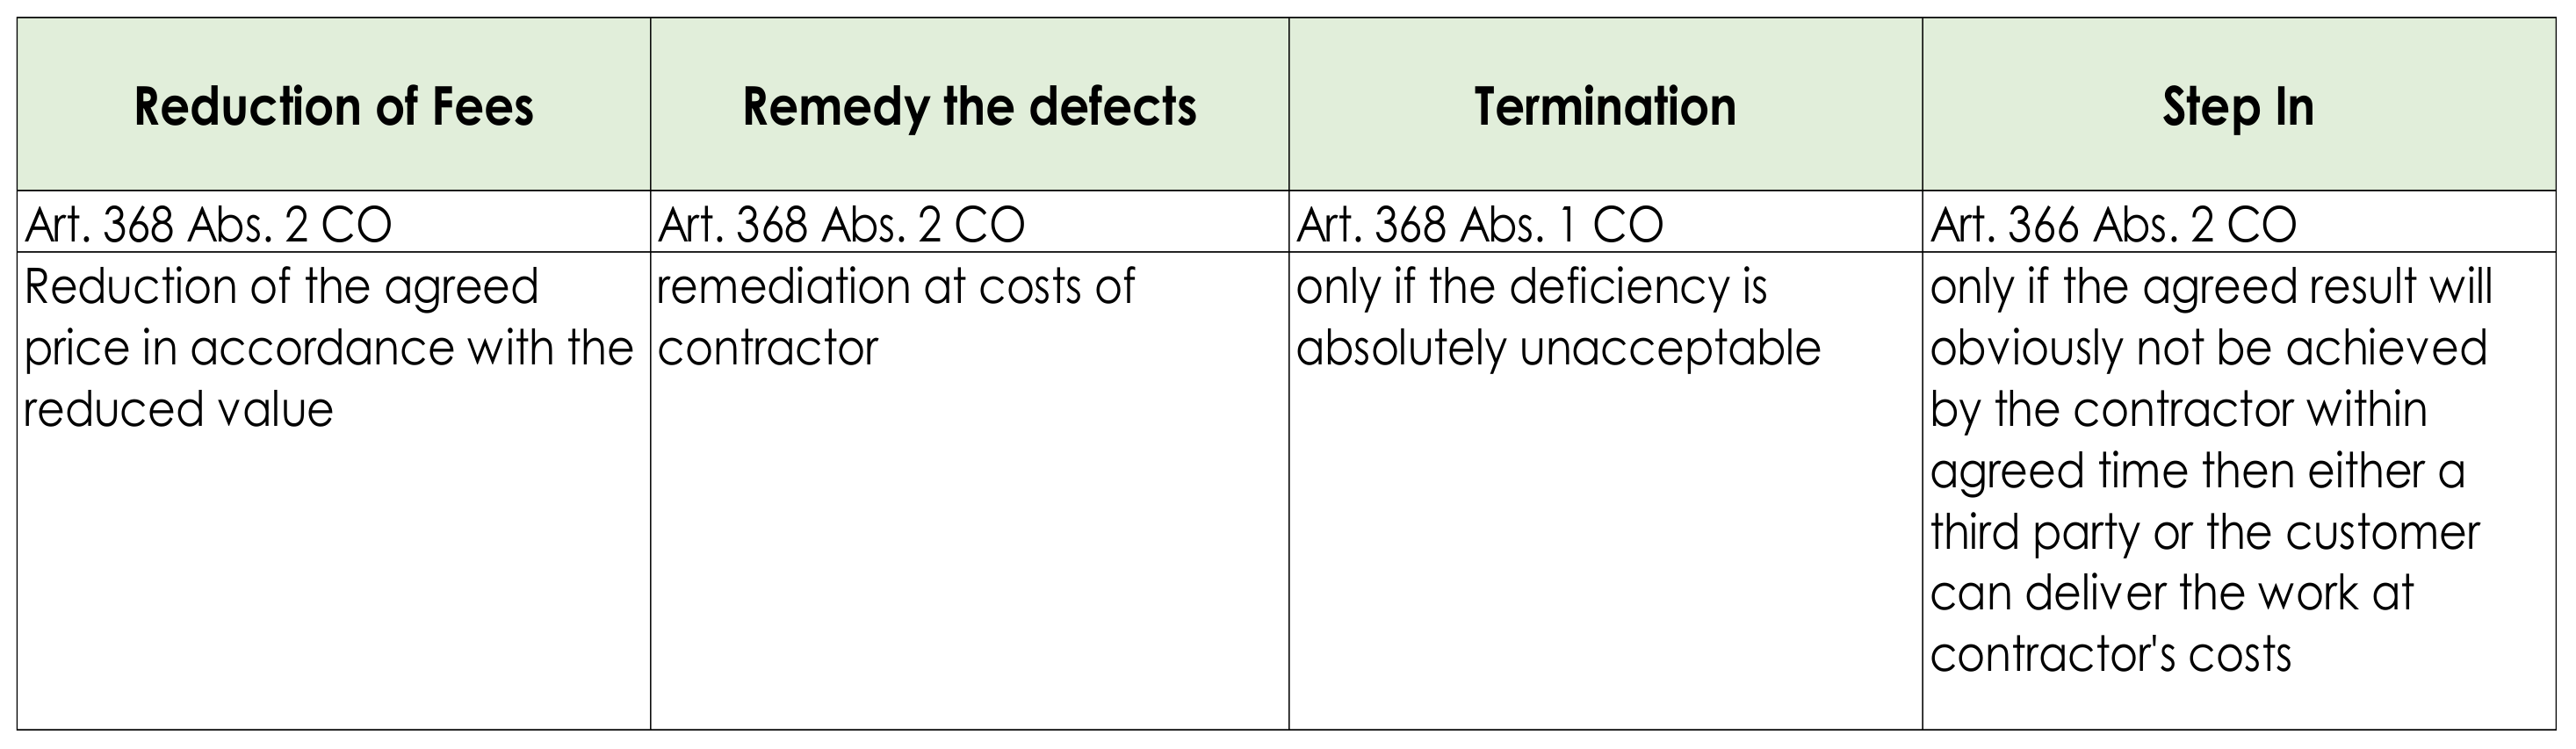
\includegraphics[width=0.9\linewidth]{img/type_contracts_service}
\end{center}
The term of a Contract for Work ends once the agreed work has been performed and delivered by the provider, and accepted by the customer.

Upon delivery the customer is required to verify whether the work has all the agreed features.

The customer may withdraw from the contract at any time before the work is completed provided he pays for work already done and indemnifies the contractor in full.

\subsection{Contract for Services (Mandate / Agency)}
Under a contract for Services the agent has
\begin{enumerate}
	\item to render the services personally unless agreed otherwise
	\item to act in accordance with the instructions provided by the customer
	\item a duty of loyalty towards the customer and duty of care as regards the services rendered
	\item to account for the services rendered
\end{enumerate}
Term and Termination may be agreed by the parties. However, a contract for Services may be terminated anytime for any reason with immediate effect (Art 404 CO). This termination right may not be waived or modified, and no fixed term may be validly agreed upon. If terminated at an improper time, the terminating party is liable for damages.

\subsection{Comparison Between Contracts to Perform Work}
\begin{center}
	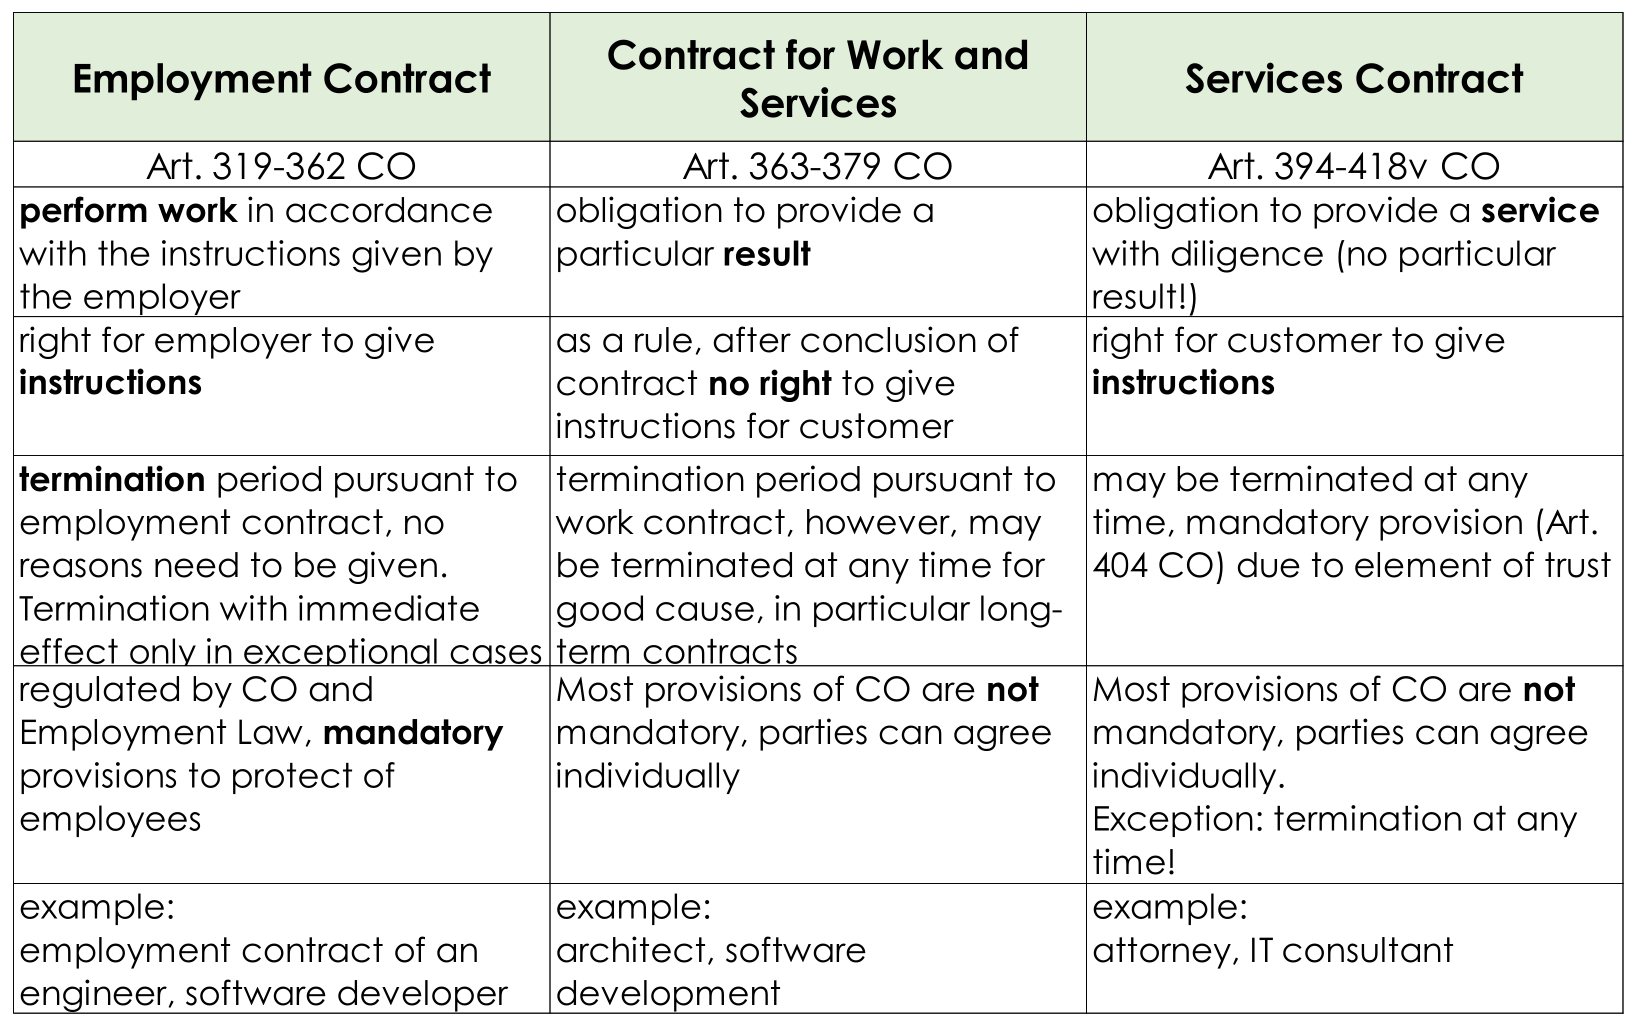
\includegraphics[width=0.9\linewidth]{img/comparison_contracts_work}
\end{center}

\subsection{IT related Contracts}
\begin{tabularx}{\linewidth}{X X}
	\hline
	\textbf{Description} & \textbf{Type} \\
	\hline
	Procurement (Hardware Software) & Purchase / License \\
	Software Development & Contract for Work \\
	Software Licensing & Sui generis \\
	Software Support / Maintenance and Service Level Agreements & Contract for Work / Contract for Services \\
	IT-Consulting & Contract for Services \\
	System Integration & Contract for Work \\
	IT-Outsourcing & Contract for Work / Contract for Services \\
	SAAS / PAAS / IAAS & Contract for Work / Contract for Services \\
	Management of ICT resources & Contract for Services \\
	Source code escrow & Contract for Services
\end{tabularx}

\subsubsection{Software Licenses}
\begin{enumerate}
	\item \textbf{simple license} Licensor can use, multiple party can license
	\item \textbf{exclusive license} Solely the licensing party can use
	\item \textbf{sole license} Only licensor and licensing party can use
\end{enumerate}

\subsubsection{Outsourcing}
\begin{enumerate}
	\item No defined contract type according to Swiss law
	\item Only few mandatory provisions in Swiss law
	\item Is getting standardised (Anglo-American contracting approach)
	\item Beware of regulatory requirements
	\item No specific form required
	\item Any contract should always be clear and self-explanatory
	\item In a long term relationship, the contract should be balanced, there is no point in a bleeding provider
	\item In a long term relationship, there is the need for proper governance to ensure the parties can communicate through a proper channel and work together effectively
\end{enumerate}
\begin{center}
	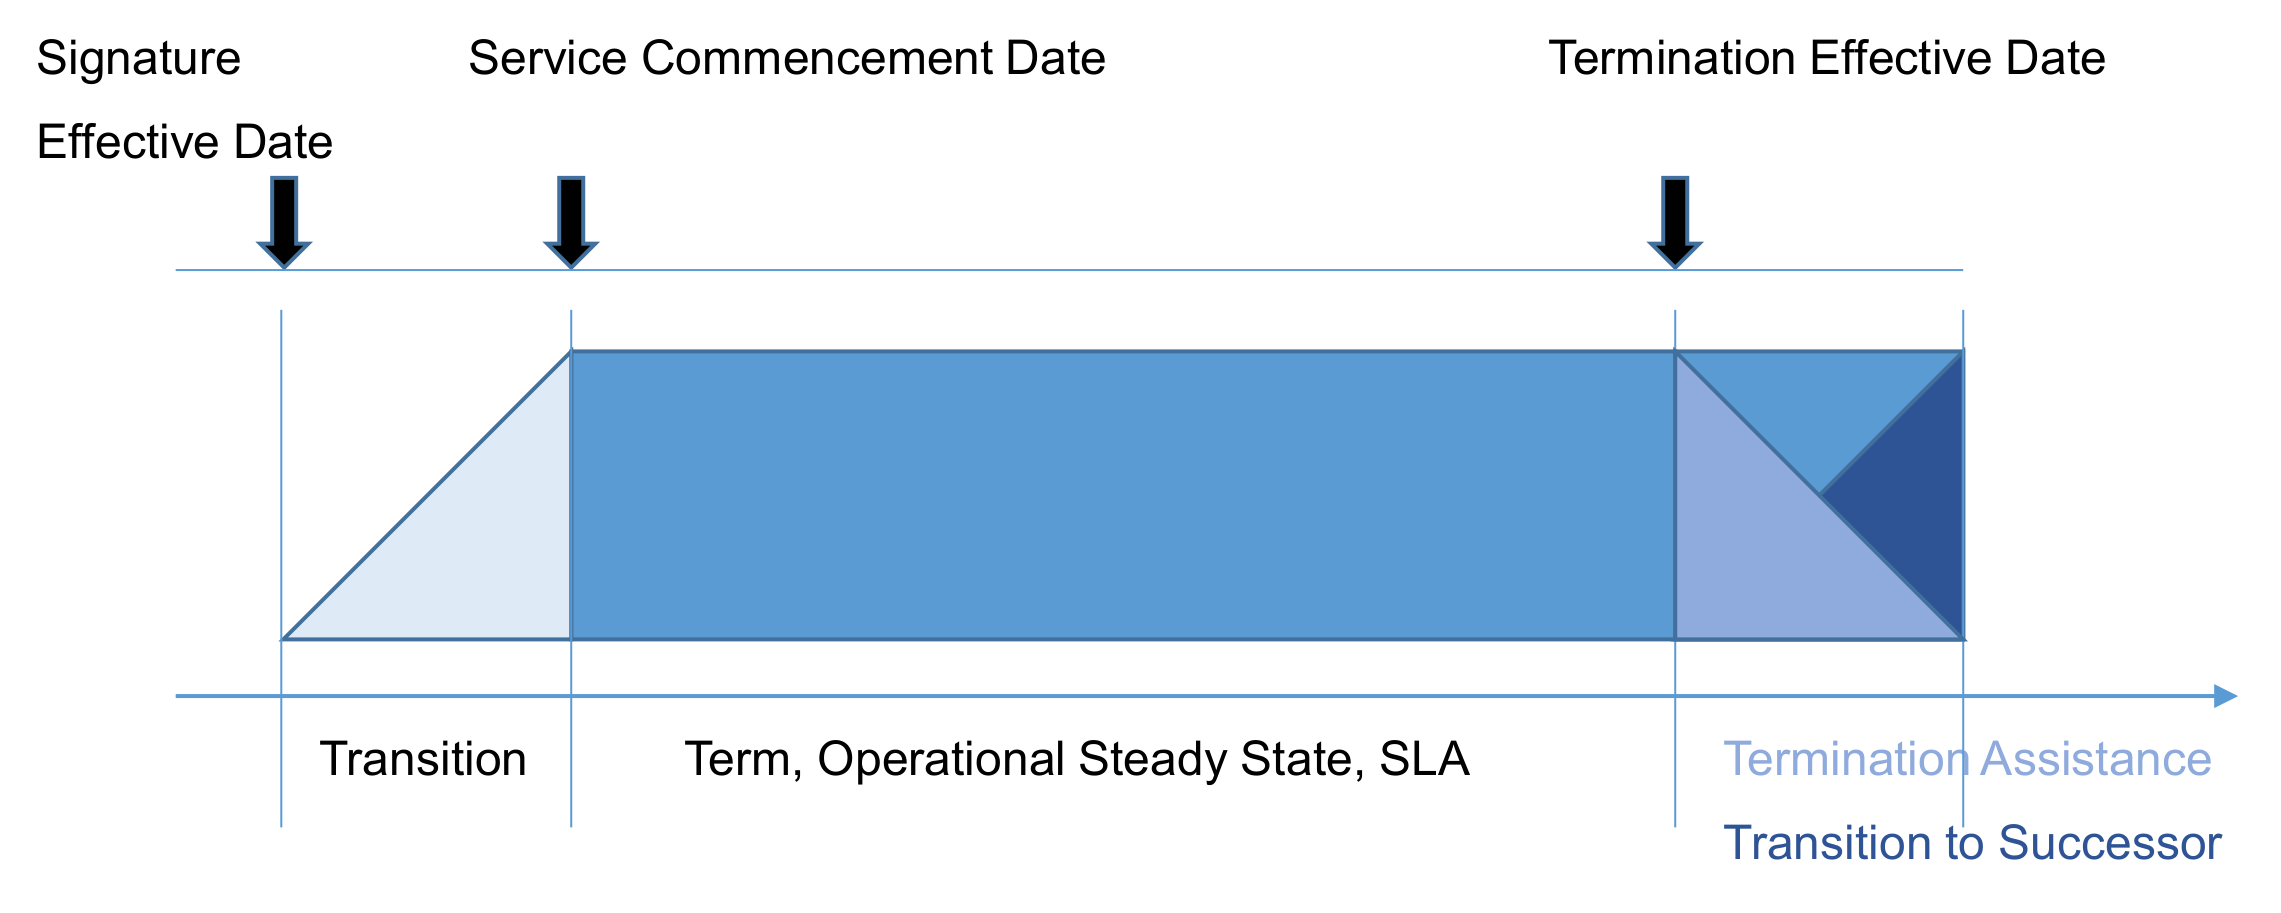
\includegraphics[width=\linewidth]{img/outsourcing_state}
\end{center}

\subsubsection{Agile}
Main differences to classic software development contracts
\begin{enumerate}
	\item The result and the detailed specifications are not defined from the outset. Rather a vision of a product is defined. The specifications are then developed jointly over time.
	\item There is no final delivery of a specific result that the customer then accepts, rather the customer needs to verify the partial deliveries and accept these on an incremental basis.
	\item The customer needs to appoint personnel with the requisite expertise and availability, as governance is key for success.
\end{enumerate}

\section{Criminal Aspects of Privacy}
Monopoly of public power as a stabilising, cultural achievement. But only if the monopoly is democratically legitimated, and if the procedures and sanctions are predictable, legally controllable and appealable. There exists a strict democratic principle of "nulla poena sine lege" (No punishment without law).

The aim of criminal sanctions are, among other things \textbf{deterrence} and \textbf{individual improvement}. The latter is the reason why children and adolescents are treated differently (juvenile criminal law).

\subsection{Criminal Liability}
Prerequisites are
\begin{enumerate}
	\item human action
	\item the constituent elements of the offence (\textbf{objective/subjective})
	\item unlawfulness
	\item criminal liability of the offender
	\item threatened with penalty/sanction (\textbf{legal base})
\end{enumerate}

\subsection{Sanctions}
\textbf{Punishments} (Bestrafungen)
\begin{itemize}
	\item Imprisonment
	\item Daily allowances and Fines
	\item Charitable work
\end{itemize}

\vspace{1em}
\noindent
\textbf{Measures} (Sanktionen)
\begin{itemize}
	\item Therapeutic measures
	\item Custody
	\item Other (Professional Ban, Driving Ban, Confiscation, etc.)
\end{itemize}

\subsubsection{Punishments}
\begin{itemize}
	\item Sentences: three days to 20 years, in some cases life-long
	\item Daily allowances: one to 360 daily rates
	\item Fines: in principle up to 10'000 CHF, but can be higher if required by law
	\item Non-profit Work: up to 720 hours
	\item A conditional prison sentence can be combined with an unconditional fine
	\item Several offences have an aggravating effect (increased penalty, but not simply adding up the individual penalties)
\end{itemize}

\subsection{Course of Criminal Proceedings}
\begin{itemize}
	\item Police or the Public Prosecutor (StA) becomes active
	\item Public Prosecutor has the lead in the investigation
	\item Public Prosecutor has the task of investigating incriminating and exoneration aspects
	\item Public Prosecutor decides whether to refer the case to the criminal court for evaluation or not
	\item Public Prosecutor has the criminal competence in simple cases. It issues a penal order for this purpose. Objection can be submitted within 10 days.
\end{itemize}

\subsection{Typical Cyber Crimes}
\begin{itemize}[noitemsep]
	\item Unauthorized data procurement (Unbefugte Datenbeschaffung 143bis StGB)
	\item Unauthorized intrusion into data precessing systems (Unbefugtes Eindringen in Datenverarbeitungssystem 143bis StGB)
	\item Data corruption (Datenbeschädigung 144bis StGB)
	\item Fraudulent abuse of a data processing system (Betrügerischer Missbrauch einer Datenverarbeitungsanlage 147 StGB)
	\item Production and marketing of materials for the unauthorised decoding of coded offers (Herstellen und Inverkehrbringen von Materialien zur unbefugten Entschlüsselung codierter Angebote 150 StGB)
	\item Violation of manufacturing or trade secret (Verletzung des Fabrikation oder Geschäftsgeheimnisses 162 StGB)
	\item Violations of honour (Ehrverletzungen 173 ff StGB)
	\item Violation of the secrecy of correspondence (Verletzung des Schriftgeheimnisses 179 StGB)
	\item Unbefugtes Beschaffen von Personendaten (179novies StGB)
	\item Pornography (197 StGB)
	\item Disturbance of establishments serving the general public (Störung von Betrieben, die der Allgemeinheit dienen 239 StGB)
	\item Racial discrimination (Rassendiskriminierung 261bis StGB)
	\item Economic Intelligence Service (Wirtschaftlicher Nachrichtendienst 273 StGB)
\end{itemize}

\subsubsection{Unbefugte Datenbeschaffung 143bis StGB}
\begin{enumerate}[label=\arabic* ]
	\item Wer in der Absicht, sich oder einen andern \textbf{unrechtmässig} zu \textbf{bereichern}, sich oder einem andern elektronisch oder in vergleichbarer Weise gespeicherte oder übermittelte \textbf{Daten beschafft, die nicht für ihn bestimmt} und \textbf{gegen seinen unbefugten Zugriff besonders gesichert sind}, wird mit Freiheitsstrafe bis zu fünf Jahren oder Geldstrafe bestraft.
	\item Die unbefugte Datenbeschaffung zum Nachteil eines Angehörigen oder Familiengenossen wird nur auf Antrag verfolgt.
\end{enumerate}

\subsubsection{Unbefugtes Eindringen in Datenverarbeitungssystem 143bis StGB}
\begin{enumerate}[label=\arabic* ]
	\item Wer auf dem Wege von Datenübertragungseinrichtungen unbefugterweise in ein fremdes, \textbf{gegen seinen Zugriff besonders gesichertes Datenverarbeitungssystem eindringt}, wird, auf Antrag, mit Freiheitsstrafe bis zu drei Jahren oder Geldstrafe bestraft.
	\item Wer Passwörter, Programme oder andere Daten, von denen er weiss oder annehmen muss, dass sie zur Begehung einer strafbaren Handlung gemäss Absatz 1 verwendet werden sollen, in Verkehr bringt oder zugänglich macht, wird mit Freiheitsstrafe bis zu drei Jahren oder Geldstrafe bestraft.
\end{enumerate}

\subsubsection{Datenbeschädigung 144bis StGB}
\begin{enumerate}[label=\arabic* ]
	\item Wer unbefugt elektronisch oder in vergleichbarer Weise gespeicherte oder übermittelte Daten verändert, löscht oder unbrauchbar macht, wird, auf Antrag, mit Freiheitsstrafe bis zu drei Jahren oder Geldstrafe bestraft.
	
	Hat der Täter einen grossen Schaden verursacht, so kann auf Freiheitsstrafe von einem Jahr bis zu fünf Jahren erkannt werden. Die Tat wird von Amtes wegen verfolgt.
	\item Wer Programme, von denen er weiss oder annehmen muss, dass sie zu den in Ziffer 1 genannten Zwecken verwendet werden sollen, herstellt, einführt, in Verkehr bringt, anpreist, anbietet oder sonst wie zugänglich macht oder zu ihrer Herstellung Anleitung gibt, wird mit Freiheitsstrafe bis zu drei Jahren oder Geldstrafe bestraft.
	
	Handelt der Täter gewerbsmässig, so kann auf Freiheitsstrafe von einem Jahr bis zu fünf Jahren erkannt werden.
\end{enumerate}

\subsubsection{Betrügerischer Missbrauch einer Datenverarbeitungsanlage 147 StGB}
\begin{enumerate}[label=\arabic* ]
	\item Wer in der Absicht, sich oder einen andern unrechtmässig zu bereichern, \textbf{durch unrichtige, unvollständige oder unbefugte Verwendung von Daten} oder in vergleichbarer Weise auf einen elektronischen oder vergleichbaren \textbf{Datenverarbeitungs- oder Datenübermittlungsvorgang einwirkt und dadurch eine Vermögensverschiebung zum Schaden eines andern herbeiführt oder eine Vermögensverschiebung unmittelbar darnach verdeckt}, wird mit Freiheitsstrafe bis zu fünf Jahren oder Geldstrafe bestraft.
	\item Handelt der Täter gewerbsmässig, so wird er mit Freiheitsstrafe bis zu zehn Jahren oder Geldstrafe nicht unter 90 Tagessätzen bestraft.
	\item Der betrügerische Missbrauch einer Datenverarbeitungsanlage zum Nachteil eines Angehörigen oder Familiengenossen wird nur auf Antrag verfolgt.
\end{enumerate}

\subsubsection{Herstellen und Inverkehrbringen von Materialien zur unbefugten Entschlüsselung codierter Angebote 150 StGB}
\begin{enumerate}[label=\arabic* ]
	\item Wer Geräte, deren Bestandteile oder Datenverarbeitungsprogramme, die zur unbefugten Entschlüsselung codierter Rundfunkprogramme oder Fernmeldedienste bestimmt und geeignet sind, herstellt, einführt, ausführt, durchführt, in Verkehr bringt oder installiert, wird, auf Antrag, mit Busse bestraft.
	\item Versuch und Gehilfenschaft sind strafbar.
\end{enumerate}

\subsection{Offences of Libel (Ehrverletzung) Art 173,174,177 StGB}
\begin{itemize}
	\item Slander (Üble Nachrede Art 173 StGB)\\
	Der Straftatbestand hat zum Ziel, jemanden zu bestrafen, der gegenüber Dritten über eine andere Person \textbf{rufschädigende} (eng. defamatory) vorsätzlich, \textbf{wahre} (oder unvorsätzlich, gutgläubig unwahre) \textbf{Äusserungen tätigt oder weiterverbreitet}.
	
	Der Täter kann sich allerdings entlasten und bleibt straflos, wenn ihm der sogenannte Entlastungsbeweis (VSS: wahr und öffentliches Interesse) gelingt.
	
	\item Defamation (Verleumdung Art 174 StGB)\\
	Die Verleumdung ist üble Nachrede \textbf{wider besseren Wissens}. Der Täter beschuldigt oder verdächtigt eine Person gegenüber Dritten eines unehrenhaften Verhaltens oder anderer rufschädigender Tatsachen, die in Wirklichkeit nicht bestehen und somit unwahr sind. Der \underline{Entlastungsbeweis ist nicht möglich}.
	
	\item Insult (Beschimpfung Art 177 StGB)\\
	Der Beschimpfung macht sich strafbar, wenn jemand in anderer Weise durch \textbf{Wort, Schrift, Bild, Gebärde oder Tätlichkeiten in der Ehre angegriffen} wird.
\end{itemize}

\subsection{Tips from a Law Practitioner}
\begin{itemize}
	\item Don't wait in case of reporting offences, there is a deadline of 90 days (Art 31)
	\item Weighing up criminal charges versus civil law suits well (time, costs, subsequent consequences)
	\item Only private plaintiffs receive information from the investigation
	\item What is once in the interview protocol can hardly be corrected
	\item As a rule, cooperation is better than refusal to testify. But as an accused person you do not have to incriminate yourself. You have the right to keep quiet.
	\item Prepare an emergency plan for a "house search"
\end{itemize}



\end{document}
